\section{Package \bfseries \texttt{modeling}\normalfont}
% Here comes the package documentation
\subsection{Package Overview}
	
			
The modeling package is the root package for the SDM meta-model. It defines several abstract super classes which implement an extension mechanism as well as reoccuring structural features like, e.g., names of elements. The classes in this package are intended to be sub-classed by any meta-model element.	
		
	
			
		
% Here a manual modifiable file is included: modeling/graphics.tex
%
% This file has been generated by Ecore to LaTeX written in oAW Xpand
% It is save to alter this file as it WILL NOT be overwritten.
% The file is included by the main latex file in the appropriate place, not further
% actions are required
%

\begin{figure}[htbp]
  \centering
  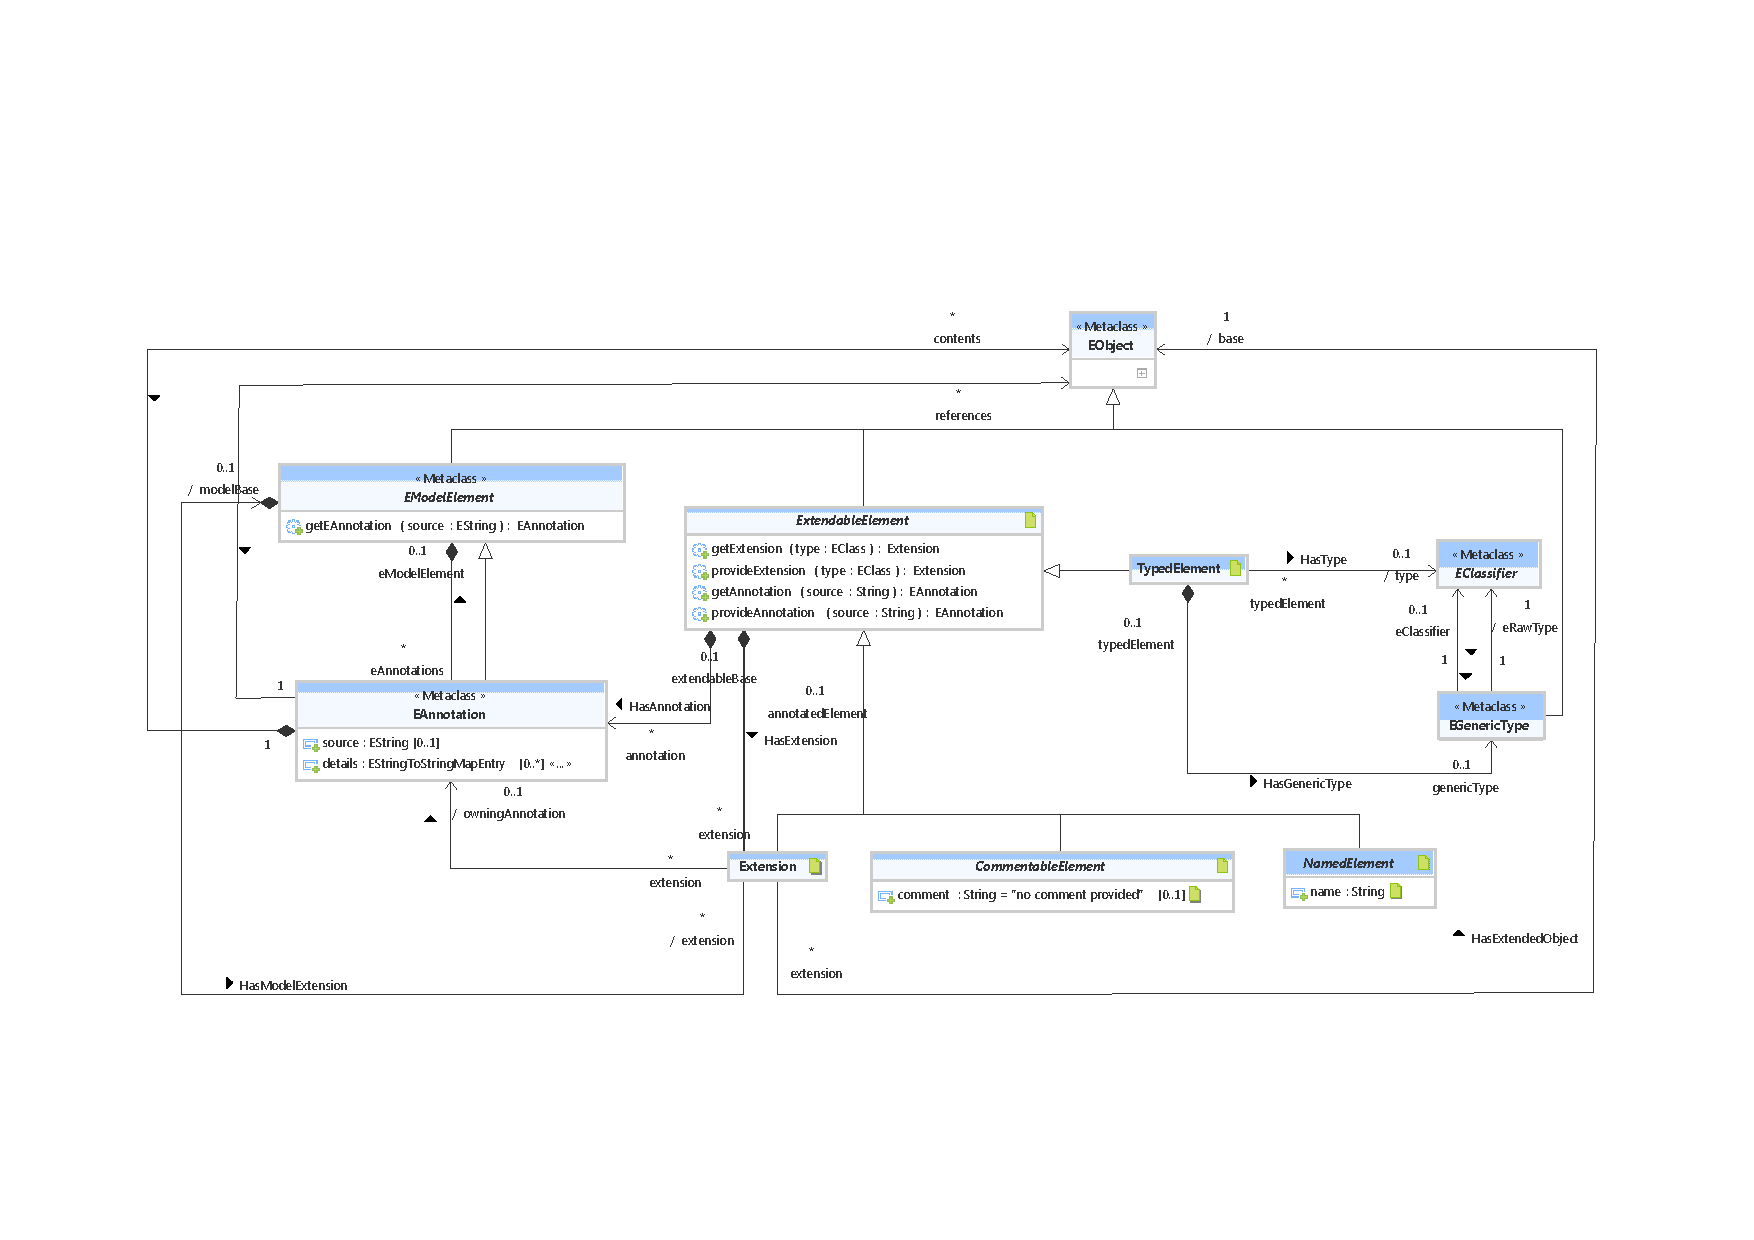
\includegraphics[width=\textheight,angle=90]{figures/A_technical-reference/packages/core/core}
  \caption{Class Structure of the \fe{core} Package}
  \label{fig:MM:modeling}
\end{figure}



\subsection{Detailed Contents Documentation}
\subsubsection{\Large{Class \bfseries \texttt{CommentableElement}\normalfont}}
\label{cls:modeling::CommentableElement} \index{3}
\paragraph{Overview}

	
			
Abstract super class for all meta-model elements that may carry a comment in form of a string.	
		
	


\begin{description}

	\item[\textbf{Class Properties}] Class \texttt{CommentableElement} has the following properties:
	\begin{description}
\item[comment : EString 			\symbol{"5B}0..1\symbol{"5D}]
\hspace{\fill}
\nopagebreak


		\todoib{Documentation missing?}
	
	\end{description}
	
	

\end{description}

\paragraph{Parent Classes}
\begin{itemize}
\item ExtendableElement see Section~\ref{cls:modeling::ExtendableElement} on Page~\pageref{cls:modeling::ExtendableElement}\end{itemize}
\subsubsection{\Large{Class \bfseries \texttt{ExtendableElement}\normalfont}}
\label{cls:modeling::ExtendableElement} \index{1}
\paragraph{Overview}

	
			
Abstract base class for the whole SDM model. The ExtendableElement specifies the extension mechanism that can be used to extend an object by an Extension containing additional attributes and references.	
		
	



\paragraph{Parent Classes}
\begin{itemize}
\item EObject\end{itemize}
\subsubsection{\Large{Class \bfseries \texttt{Extension}\normalfont}}
\label{cls:modeling::Extension} \index{2}
\paragraph{Overview}

	
			
Abstract super class for an Extension that can be defined for an object.	
		
	



\paragraph{Parent Classes}
\begin{itemize}
\item ExtendableElement see Section~\ref{cls:modeling::ExtendableElement} on Page~\pageref{cls:modeling::ExtendableElement}\end{itemize}
\subsubsection{\Large{Class \bfseries \texttt{NamedElement}\normalfont}}
\label{cls:modeling::NamedElement} \index{5}
\paragraph{Overview}

	
			
Abstract super class for all meta-model elements that carry a name. 	
		
	


\begin{description}

	\item[\textbf{Class Properties}] Class \texttt{NamedElement} has the following properties:
	\begin{description}
\item[name : EString 	]
\hspace{\fill}
\nopagebreak


	
			
The name attribute of a meta-model element.	
		
	
	\end{description}
	
	

\end{description}

\paragraph{Parent Classes}
\begin{itemize}
\item ExtendableElement see Section~\ref{cls:modeling::ExtendableElement} on Page~\pageref{cls:modeling::ExtendableElement}\end{itemize}
\subsubsection{\Large{Class \bfseries \texttt{TypedElement}\normalfont}}
\label{cls:modeling::TypedElement} \index{0}
\paragraph{Overview}

	
			
Abstract super class for all meta-model elements that are typed by means of an EClassifier or an EGenericType.	
		
	



\paragraph{Parent Classes}
\begin{itemize}
\item ExtendableElement see Section~\ref{cls:modeling::ExtendableElement} on Page~\pageref{cls:modeling::ExtendableElement}\end{itemize}
\subsubsection{\Large{Class \bfseries \texttt{Variable}\normalfont}}
\label{cls:modeling::Variable} \index{4}
\paragraph{Overview}

	
			
Represents a variable which can be, for example, an object variable, an attribute, or any other kind of variable.	
		
	


\begin{description}

	\item[\textbf{Class Properties}] Class \texttt{Variable} has the following properties:
	\begin{description}
\item[/variableName : EString 			\symbol{"5B}0..1\symbol{"5D}]
\hspace{\fill}
\nopagebreak


		\todoib{Documentation missing?}
	
	\end{description}
	
	

\end{description}

\paragraph{Parent Classes}
\begin{itemize}
\item TypedElement see Section~\ref{cls:modeling::TypedElement} on Page~\pageref{cls:modeling::TypedElement}\end{itemize}
\newpage
		


\section{Package \bfseries \texttt{modeling::activities}\normalfont}
% Here comes the package documentation
\subsection{Package Overview}
		\todoib{Documentation missing?}
	
			
		
% Here a manual modifiable file is included: activities/graphics.tex
%
% This file has been generated by Ecore to LaTeX written in oAW Xpand
% It is save to alter this file as it WILL NOT be overwritten.
% The file is included by the main latex file in the appropriate place, not further
% actions are required
%

\begin{figure}[htbp]
  \centering
  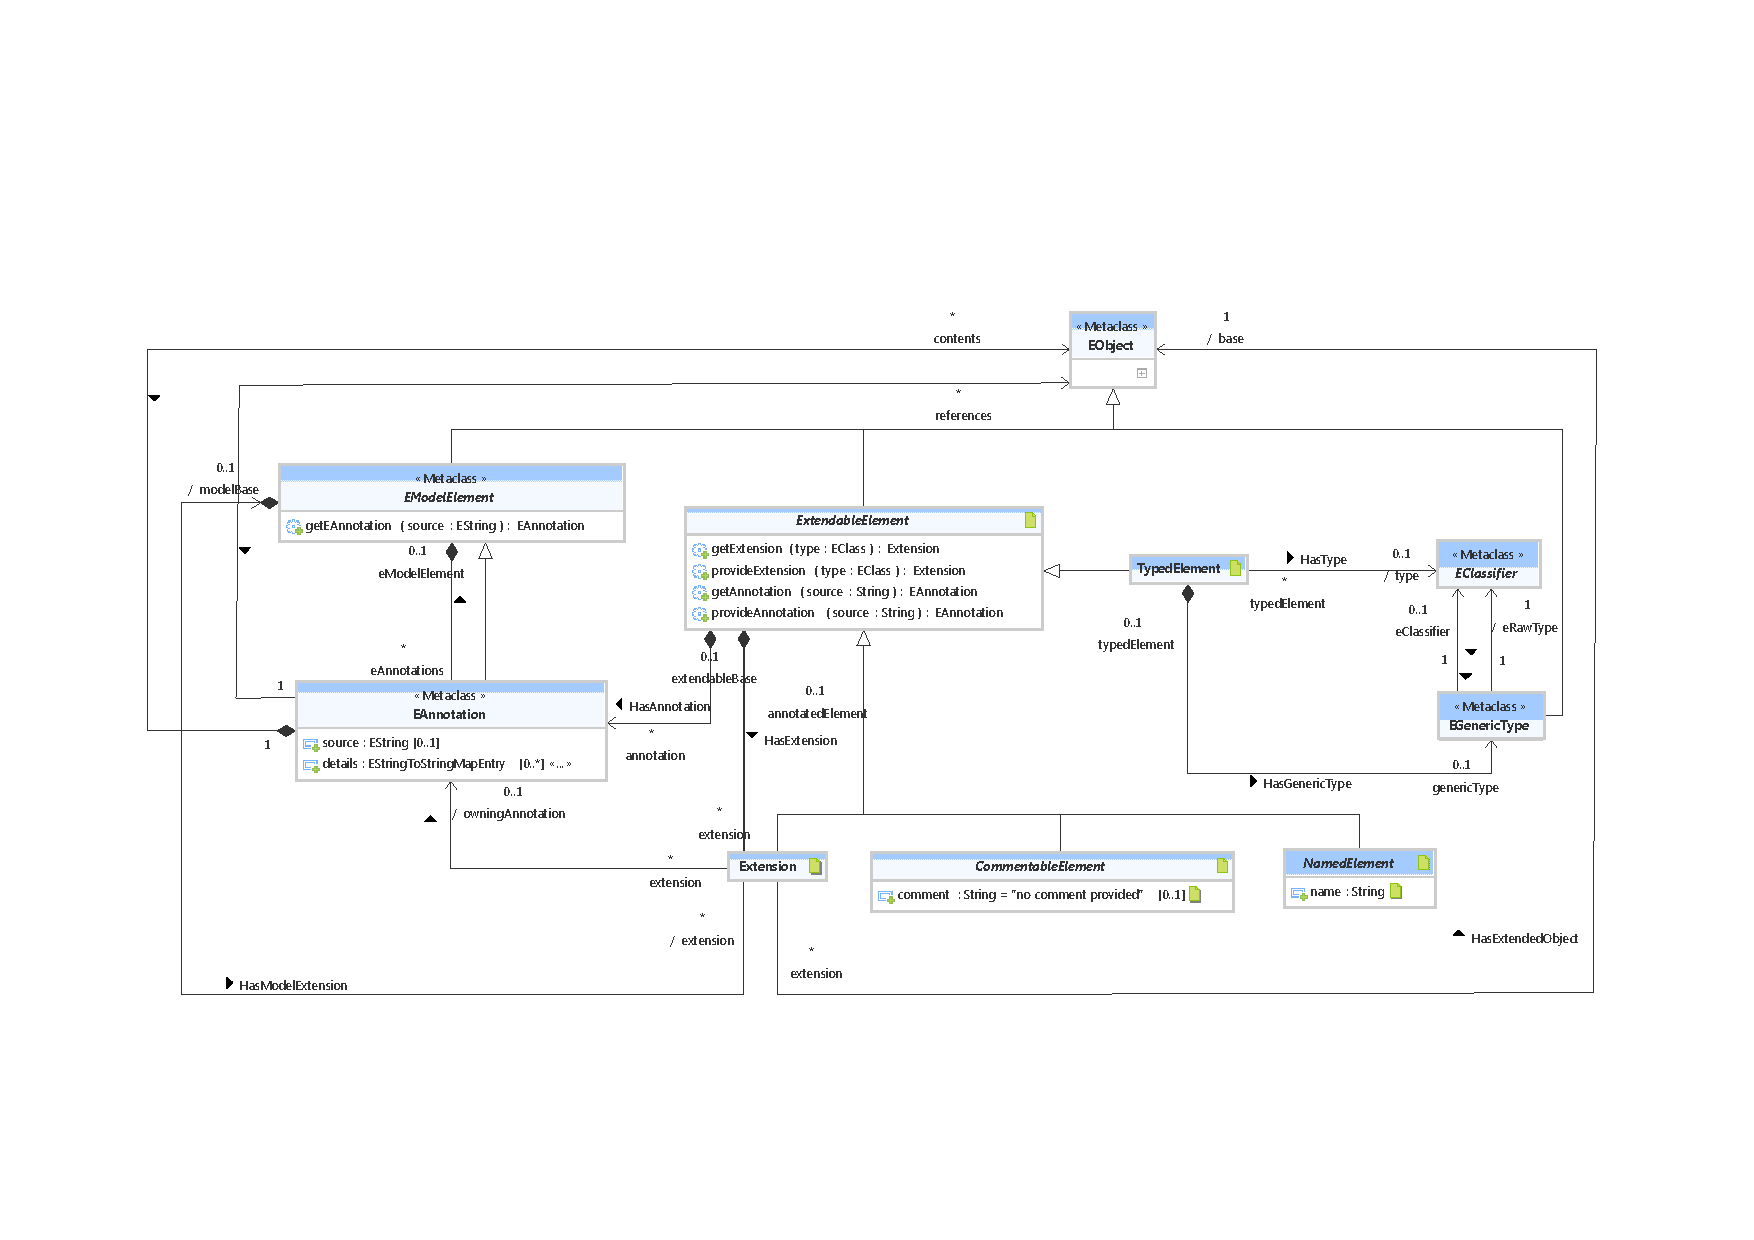
\includegraphics[width=\textheight,angle=90]{figures/A_technical-reference/packages/core/core}
  \caption{Class Structure of the \fe{core} Package}
  \label{fig:MM:modeling}
\end{figure}



\subsection{Detailed Contents Documentation}
\subsubsection{\Large{Class \bfseries \texttt{Activity}\normalfont}}
\label{cls:modeling::activities::Activity} \index{3}
\paragraph{Overview}

	
			
The diagram that describes the control flow of an operation. It is used to structure a number story patterns into a stroy diagram. Story patterns are contained in activity nodes which are connected by activity edges. In addition, there are special nodes like start, stop, and juction nodes.  	
		
	



\paragraph{Parent Classes}
\begin{itemize}
\item CommentableElement see Section~\ref{cls:modeling::CommentableElement} on Page~\pageref{cls:modeling::CommentableElement}, \item Callable see Section~\ref{cls:modeling::calls::Callable} on Page~\pageref{cls:modeling::calls::Callable}\end{itemize}
\subsubsection{\Large{Class \bfseries \texttt{ActivityCallNode}\normalfont}}
\label{cls:modeling::activities::ActivityCallNode} \index{13}
\paragraph{Overview}

	
			
The ActivityCallNode is a special ActivityNode which represents the calling of another story diagram within an activity.
To support polymorphic dispatching, multiple activities can be assigned to it (all of which must have the same call signature, i.e. matching in and out parameters). All assigned activities are then called in the given order and the first one whose precondition is fulfilled is executed (Chain of Responsibilty).	
		
	



\paragraph{Parent Classes}
\begin{itemize}
\item ActivityNode see Section~\ref{cls:modeling::activities::ActivityNode} on Page~\pageref{cls:modeling::activities::ActivityNode}, \item Invocation see Section~\ref{cls:modeling::calls::Invocation} on Page~\pageref{cls:modeling::calls::Invocation}\end{itemize}
\subsubsection{\Large{Class \bfseries \texttt{ActivityEdge}\normalfont}}
\label{cls:modeling::activities::ActivityEdge} \index{1}
\paragraph{Overview}

	
			
The ActivityEdge represents the control flow in an activity. It is a dericted connection from one activity to another one. There exist different kinds of activity edges which are differentiated by the guard attribute.	
		
	


\begin{description}

	\item[\textbf{Class Properties}] Class \texttt{ActivityEdge} has the following properties:
	\begin{description}
\item[guard : EdgeGuard 	]
see Section~\ref{cls:modeling::activities::EdgeGuard} on Page~\pageref{cls:modeling::activities::EdgeGuard}\hspace{\fill}
\nopagebreak


	
			
The guard defines the kind of the activity edge. The possible kinds of guards are specified by the EdgeGuard enum.	
		
	
	\end{description}
	
	\item[\textbf{Class References}] Class \texttt{ActivityEdge} has the following references:
	\begin{description}
\item[guardException : ExceptionVariable 			\symbol{"5B}0..$*$\symbol{"5D}]
see Section~\ref{cls:modeling::activities::ExceptionVariable} on Page~\pageref{cls:modeling::activities::ExceptionVariable}\hspace{\fill}
\nopagebreak


	
			
Declares variables representing the Exceptions that lead to firing this transition.	
		
	
\item[guardExpression : Expression 			\symbol{"5B}0..1\symbol{"5D}]
see Section~\ref{cls:modeling::expressions::Expression} on Page~\pageref{cls:modeling::expressions::Expression}\hspace{\fill}
\nopagebreak


	
			
Points to an expression in case the transition guard is BOOL. The expression has to evaulate to a boolean value.	
		
	
\item[owningActivity : Activity 	]
see Section~\ref{cls:modeling::activities::Activity} on Page~\pageref{cls:modeling::activities::Activity}\hspace{\fill}
\nopagebreak


	
			
Points to the activity this ActivityEdge is contained in.	
		
	
\item[source : ActivityNode 	]
see Section~\ref{cls:modeling::activities::ActivityNode} on Page~\pageref{cls:modeling::activities::ActivityNode}\hspace{\fill}
\nopagebreak


	
			
The source node of this ActivityEdge.	
		
	
\item[target : ActivityNode 	]
see Section~\ref{cls:modeling::activities::ActivityNode} on Page~\pageref{cls:modeling::activities::ActivityNode}\hspace{\fill}
\nopagebreak


	
			
The target node of this ActivityEdge.	
		
	
	\end{description}
	

\end{description}

\paragraph{Parent Classes}
\begin{itemize}
\item ExtendableElement see Section~\ref{cls:modeling::ExtendableElement} on Page~\pageref{cls:modeling::ExtendableElement}\end{itemize}
\subsubsection{\Large{Class \bfseries \texttt{ActivityNode}\normalfont}}
\label{cls:modeling::activities::ActivityNode} \index{2}
\paragraph{Overview}

	
			
Abstract super class for all kinds of nodes that may be added to an activity. This class provides the basic functionality of connecting the activity nodes in the activity by ActivityEdges.	
		
	



\paragraph{Parent Classes}
\begin{itemize}
\item NamedElement see Section~\ref{cls:modeling::NamedElement} on Page~\pageref{cls:modeling::NamedElement}, \item CommentableElement see Section~\ref{cls:modeling::CommentableElement} on Page~\pageref{cls:modeling::CommentableElement}\end{itemize}
\subsubsection{\Large{Enumeration \bfseries \texttt{EdgeGuard}\normalfont}}
\label{cls:modeling::activities::EdgeGuard} \index{modeling::activities!EdgeGuard}
\paragraph{Overview}
	
			
This enum is used to model different kinds of activity edges. 	
		
	


\begin{description}

	\item[\textbf{Enum Properties}] Enumeration \texttt{EdgeGuard} has the following literals:

	\begin{description}
		
		\item[NONE = 0]
		\hspace{\fill}
		\nopagebreak
		
No guard, only one outgoing activity edge of this kind is supported per activity node. If an edge with EdgeGuard NONE is used, it must be the only edge leaving a state.	

		\item[SUCCESS = 1]
		\hspace{\fill}
		\nopagebreak
		
Edge will be taken if execution of the souce activity node was successful, e.g., a story pattern was matched successfully. There must be another edge leaving the same node which is of kind FAILURE.	

		\item[FAILURE = 2]
		\hspace{\fill}
		\nopagebreak
		
Edge will be taken if execution of the source activity node was not successful, e.g., a story pattern could not be matched. There must be another edge leaving the same node which is of kind SUCCESS	

		\item[EACH\_TIME = 3]
		\hspace{\fill}
		\nopagebreak
		
Edge may only leave a StoryNode whose forEach attribute is true. It will be taken for each match that can be identified for the story pattern in the foreach StoryNode. There must be another edge leaving the same node which is of kind END	

		\item[END = 4]
		\hspace{\fill}
		\nopagebreak
		
Edge may only leave a StoryNode whose forEach attribute is true. It will be taken if no more fresh matches for the story pattern in the foreach node can be found.	

		\item[ELSE = 5]
		\hspace{\fill}
		\nopagebreak
		
Complement to the BOOL guard, ELSE may only be used if at least one BOOL activity edge leaves the same state. The edge will be taken if none of the BOOL guards can be evaluated to true	

		\item[BOOL = 6]
		\hspace{\fill}
		\nopagebreak
		
An activity edge specifying a boolean guard using variables that have been previously used in the activity. Edge will be taken if the guardExpression of the activity edge evaluates to true. More than one BOOL edge is allowed to leave an activity node.	

		\item[EXCEPTION = 7]
		\hspace{\fill}
		\nopagebreak
		
An EXCEPTION edge will be taken if an exception of the  type defined by the ExceptionVariable connected to the activity edge occured while executing the source activity node of the edge. More than one edge of kind EXCEPTION is allowed to leave a node.	

		\item[FINALLY = 8]
		\hspace{\fill}
		\nopagebreak
		
An activity edge of kind FINALLY may only leave an activity node that has at least one other outgoing edge of kind EXCEPTION. The finally edge will be taken after the source node has been executed and after, possibly, the EXCEPTION edge has been taken.	
 
	\end{description}

\end{description}



\subsubsection{\Large{Class \bfseries \texttt{ExceptionVariable}\normalfont}}
\label{cls:modeling::activities::ExceptionVariable} \index{0}
\paragraph{Overview}

	
			
Declares a variable representing an Exception that leads to firing a transition (ActivityEdge). Can only be applied to ActivityEdge whose guard is set to EXCEPTION.	
		
	


\begin{description}

	\item[\textbf{Class Properties}] Class \texttt{ExceptionVariable} has the following properties:
	\begin{description}
\item[name : EString 	]
\hspace{\fill}
\nopagebreak


	
			
Specifies the name of the declared exception variable.	
		
	
	\end{description}
	
	\item[\textbf{Class References}] Class \texttt{ExceptionVariable} has the following references:
	\begin{description}
\item[activityEdge : ActivityEdge 	]
see Section~\ref{cls:modeling::activities::ActivityEdge} on Page~\pageref{cls:modeling::activities::ActivityEdge}\hspace{\fill}
\nopagebreak


	
			
Specifies the transition (activity edge) where the exception variable is declared.	
		
	
\item[exceptionType : EClassifier 			\symbol{"5B}0..$*$\symbol{"5D}]
\hspace{\fill}
\nopagebreak


	
			
Specifies the type of the declared exception variable.	
		
	
\item[genericExceptionType : EGenericType 			\symbol{"5B}0..$*$\symbol{"5D}]
\hspace{\fill}
\nopagebreak


		\todoib{Documentation missing?}
	
	\end{description}
	

\end{description}

\paragraph{Parent Classes}
\begin{itemize}
\item Variable see Section~\ref{cls:modeling::Variable} on Page~\pageref{cls:modeling::Variable}\end{itemize}
\subsubsection{\Large{Class \bfseries \texttt{JunctionNode}\normalfont}}
\label{cls:modeling::activities::JunctionNode} \index{9}
\paragraph{Overview}

	
			
A JunctionNode represents a pseudo-activity which is used for branching and merging the control flow in an activity. It is visualized by a diamond shaped figure.	
		
	



\paragraph{Parent Classes}
\begin{itemize}
\item ActivityNode see Section~\ref{cls:modeling::activities::ActivityNode} on Page~\pageref{cls:modeling::activities::ActivityNode}\end{itemize}
\subsubsection{\Large{Class \bfseries \texttt{MatchingStoryNode}\normalfont}}
\label{cls:modeling::activities::MatchingStoryNode} \index{5}
\paragraph{Overview}

	
			
A MatchingStoryNode may only contain a MatchingPattern which does not change the graph. I.e., no element contained in this activity carries a create or destroy annotation. Thus, after executing a MatchingStoryNode, the underlying graph is guaranteed to be unchanged.	
		
	



\paragraph{Parent Classes}
\begin{itemize}
\item StoryNode see Section~\ref{cls:modeling::activities::StoryNode} on Page~\pageref{cls:modeling::activities::StoryNode}\end{itemize}
\subsubsection{\Large{Class \bfseries \texttt{ModifyingStoryNode}\normalfont}}
\label{cls:modeling::activities::ModifyingStoryNode} \index{14}
\paragraph{Overview}

	
			
A ModifyingStoryNode contains a story pattern which may change the underlying graph upon execution.	
		
	



\paragraph{Parent Classes}
\begin{itemize}
\item StoryNode see Section~\ref{cls:modeling::activities::StoryNode} on Page~\pageref{cls:modeling::activities::StoryNode}\end{itemize}
\subsubsection{\Large{Class \bfseries \texttt{OperationExtension}\normalfont}}
\label{cls:modeling::activities::OperationExtension} \index{4}
\paragraph{Overview}

	
			
An OperationExtension is a stand-in for an EOperation in our model. It is necessary because we cannot change the type EOperation. Thus, OperationExtension points to an EOperation but adds the reference to an Activity that describes the operations behavior.	
		
	



\paragraph{Parent Classes}
\begin{itemize}
\item Extension see Section~\ref{cls:modeling::Extension} on Page~\pageref{cls:modeling::Extension}, \item Callable see Section~\ref{cls:modeling::calls::Callable} on Page~\pageref{cls:modeling::calls::Callable}\end{itemize}
\subsubsection{\Large{Class \bfseries \texttt{StartNode}\normalfont}}
\label{cls:modeling::activities::StartNode} \index{10}
\paragraph{Overview}

	
			
The start node of an activity defines the starting point for the execution of the activity.	
		
	



\paragraph{Parent Classes}
\begin{itemize}
\item ActivityNode see Section~\ref{cls:modeling::activities::ActivityNode} on Page~\pageref{cls:modeling::activities::ActivityNode}\end{itemize}
\subsubsection{\Large{Class \bfseries \texttt{StatementNode}\normalfont}}
\label{cls:modeling::activities::StatementNode} \index{11}
\paragraph{Overview}

	
			
A statement node is a node that just contains an expression defining its behavior. In combination with a textual expression, arbitrary souce code might be added by using StatementNodes.	
		
	



\paragraph{Parent Classes}
\begin{itemize}
\item ActivityNode see Section~\ref{cls:modeling::activities::ActivityNode} on Page~\pageref{cls:modeling::activities::ActivityNode}\end{itemize}
\subsubsection{\Large{Class \bfseries \texttt{StopNode}\normalfont}}
\label{cls:modeling::activities::StopNode} \index{12}
\paragraph{Overview}

	
			
At a StopNode, the execution of an activity terminates. If the activity specifies any out-parameters, they have to be bound to a return expression.	
		
	


\begin{description}

	\item[\textbf{Class Properties}] Class \texttt{StopNode} has the following properties:
	\begin{description}
\item[flowStopOnly : EBoolean 	]
\hspace{\fill}
\nopagebreak


	
			
true if subactivity is stopped, but not the whole control flow	
		
	
	\end{description}
	
	\item[\textbf{Class References}] Class \texttt{StopNode} has the following references:
	\begin{description}
\item[/returnValue : Expression 			\symbol{"5B}0..1\symbol{"5D}]
see Section~\ref{cls:modeling::expressions::Expression} on Page~\pageref{cls:modeling::expressions::Expression}\hspace{\fill}
\nopagebreak


	
			
Convenience method when dealing with activities that implement an EOperation. In this case, only one out parameter is supported. This attributes then returns the first out parameter.	
		
	
\item[returnValues : Expression 			\symbol{"5B}0..$*$\symbol{"5D}]
see Section~\ref{cls:modeling::expressions::Expression} on Page~\pageref{cls:modeling::expressions::Expression}\hspace{\fill}
\nopagebreak


	
			
Defines the return values of the activity. These return values will be assigned to the out-parameters.	
		
	
	\end{description}
	

\end{description}

\paragraph{Parent Classes}
\begin{itemize}
\item ActivityNode see Section~\ref{cls:modeling::activities::ActivityNode} on Page~\pageref{cls:modeling::activities::ActivityNode}\end{itemize}
\subsubsection{\Large{Class \bfseries \texttt{StoryNode}\normalfont}}
\label{cls:modeling::activities::StoryNode} \index{6}
\paragraph{Overview}

	
			
An activity node containing a story pattern.	
		
	


\begin{description}

	\item[\textbf{Class Properties}] Class \texttt{StoryNode} has the following properties:
	\begin{description}
\item[forEach : EBoolean 	]
\hspace{\fill}
\nopagebreak


	
			
Specifies whether just one match should be found for the contained pattern (forEach  = false) or whether all matches should be found (forEach = true).	
		
	
	\end{description}
	
	\item[\textbf{Class References}] Class \texttt{StoryNode} has the following references:
	\begin{description}
\item[/storyPattern : StoryPattern 	]
see Section~\ref{cls:modeling::patterns::StoryPattern} on Page~\pageref{cls:modeling::patterns::StoryPattern}\hspace{\fill}
\nopagebreak


	
			
	
		
	
	\end{description}
	

\end{description}

\paragraph{Parent Classes}
\begin{itemize}
\item ActivityNode see Section~\ref{cls:modeling::activities::ActivityNode} on Page~\pageref{cls:modeling::activities::ActivityNode}\end{itemize}
\subsubsection{\Large{Class \bfseries \texttt{StructuredNode}\normalfont}}
\label{cls:modeling::activities::StructuredNode} \index{7}
\paragraph{Overview}

	
			
A structured node is a node that contains several other activities.	
		
	



\paragraph{Parent Classes}
\begin{itemize}
\item ActivityNode see Section~\ref{cls:modeling::activities::ActivityNode} on Page~\pageref{cls:modeling::activities::ActivityNode}\end{itemize}
\newpage
		


\section{Package \bfseries \texttt{modeling::activities::expressions}\normalfont}
% Here comes the package documentation
\subsection{Package Overview}
		\todoib{Documentation missing?}
	
			



\subsection{Detailed Contents Documentation}
\subsubsection{\Large{Class \bfseries \texttt{ExceptionVariableExpression}\normalfont}}
\label{cls:modeling::activities::expressions::ExceptionVariableExpression} \index{0}
\paragraph{Overview}

	
			
Represents the value of an exception variable declared as a transition guard (the guard of an activity edge).	
		
	



\paragraph{Parent Classes}
\begin{itemize}
\item Expression see Section~\ref{cls:modeling::expressions::Expression} on Page~\pageref{cls:modeling::expressions::Expression}\end{itemize}
\newpage
		


\section{Package \bfseries \texttt{modeling::calls}\normalfont}
% Here comes the package documentation
\subsection{Package Overview}
	
			
This package contains all classes for modeling calls to activities and EOperations
from within an activity.	
		
	
			
		
% Here a manual modifiable file is included: calls/graphics.tex
%
% This file has been generated by Ecore to LaTeX written in oAW Xpand
% It is save to alter this file as it WILL NOT be overwritten.
% The file is included by the main latex file in the appropriate place, not further
% actions are required
%

\begin{figure}[htbp]
  \centering
  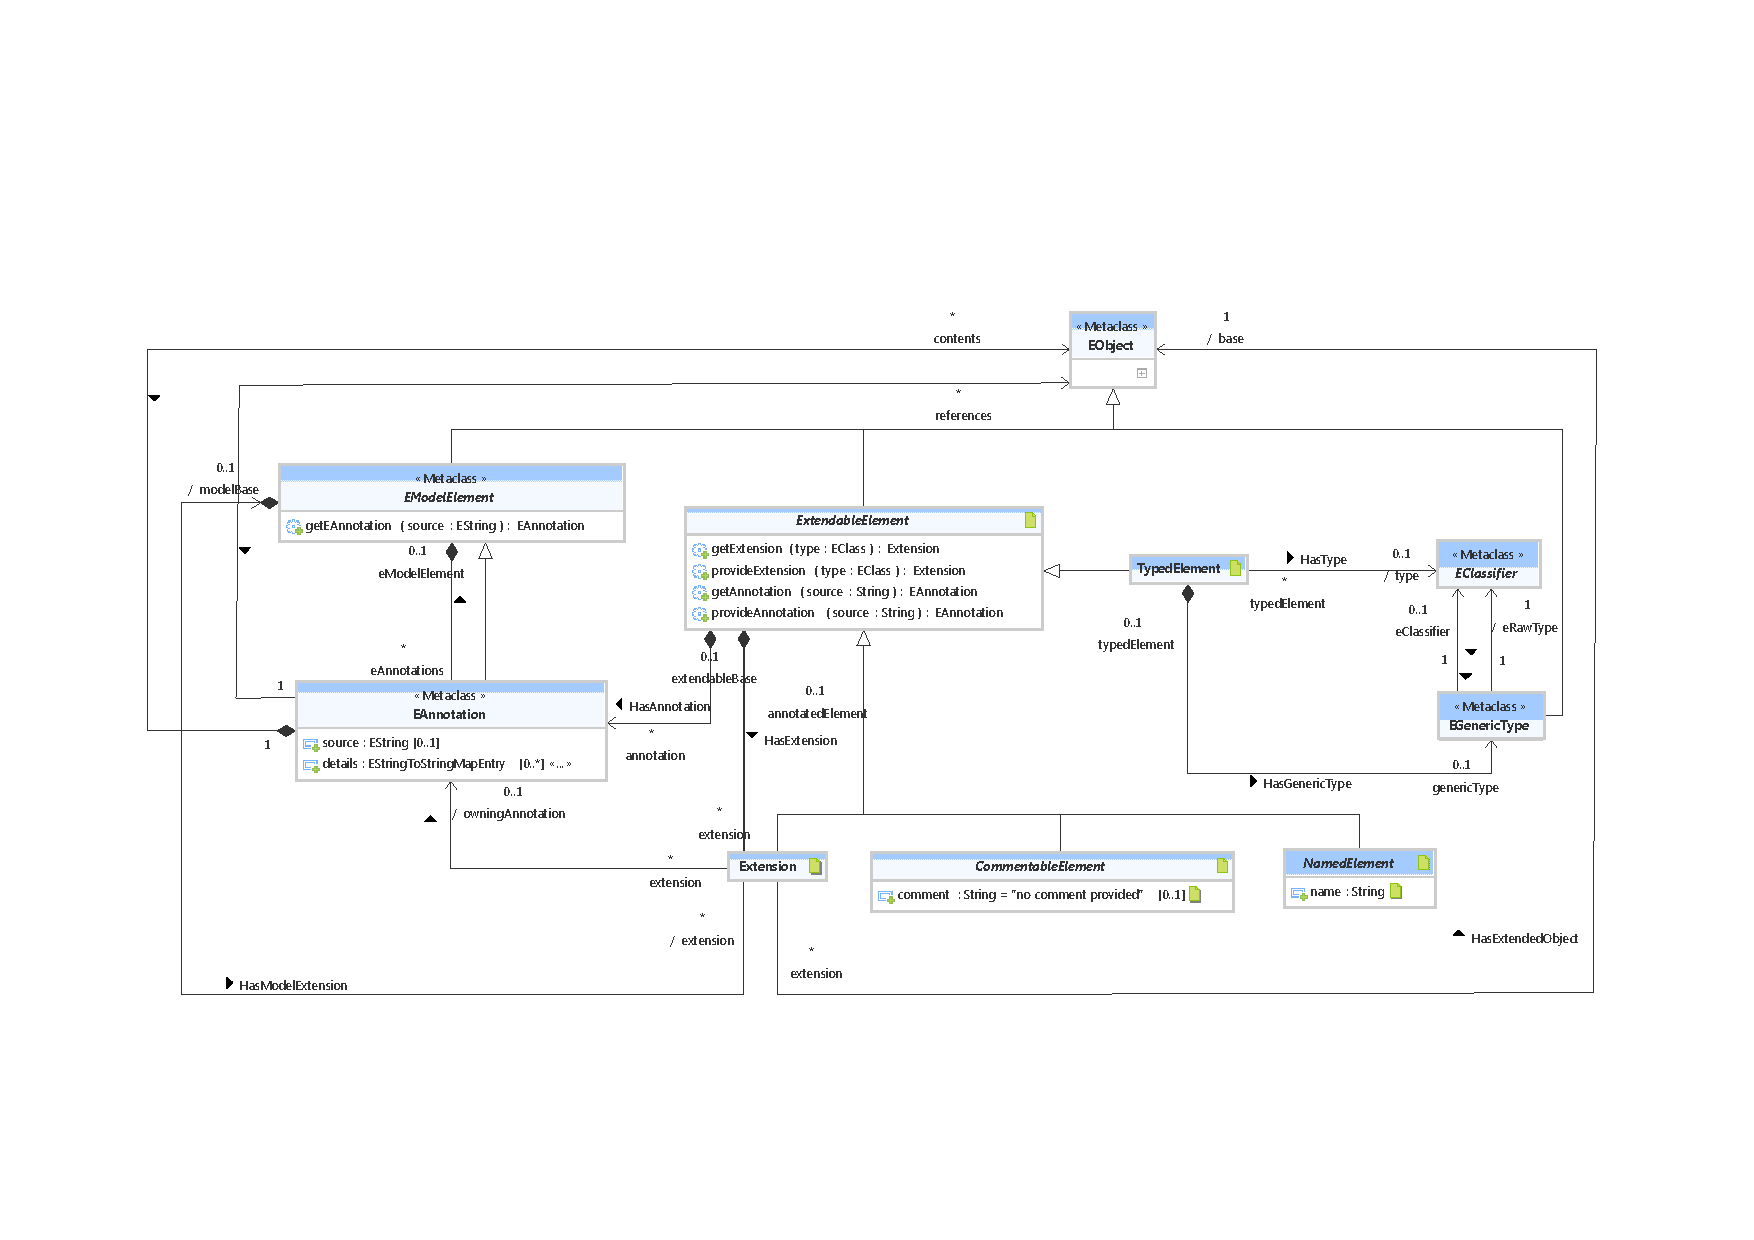
\includegraphics[width=\textheight,angle=90]{figures/A_technical-reference/packages/core/core}
  \caption{Class Structure of the \fe{core} Package}
  \label{fig:MM:modeling}
\end{figure}



\subsection{Detailed Contents Documentation}
\subsubsection{\Large{Class \bfseries \texttt{Callable}\normalfont}}
\label{cls:modeling::calls::Callable} \index{4}
\paragraph{Overview}

	
			
An entity which can be called by an Invocation. A Callable can have a number of (ordered) parameters which are either in or out parameters. In the case of activities, the number of in and out parameters is unbounded, whereas OperationExtensions and OpaqueCallables can only have one out parameter (This is enforced by an OCL constraint).	
		
	



\paragraph{Parent Classes}
\begin{itemize}
\item CommentableElement see Section~\ref{cls:modeling::CommentableElement} on Page~\pageref{cls:modeling::CommentableElement}\end{itemize}
\subsubsection{\Large{Class \bfseries \texttt{Invocation}\normalfont}}
\label{cls:modeling::calls::Invocation} \index{0}
\paragraph{Overview}

	
			
Superclass for invocations of behavior which is specified elsewhere, e.g. in methods (MethodCallExpression) or activities (ActivityCallNode). An invocation has one parameter binding for each parameter (in or out) of the called method/activity. For Callables which are contained in the model (i.e. Activities and OperationExtensions) the Invocation directly points to the callee. OpaqueCallables are directly referenced by (and contained in) the MethodCallExpressions.	
		
	



\paragraph{Parent Classes}
\begin{itemize}
\item CommentableElement see Section~\ref{cls:modeling::CommentableElement} on Page~\pageref{cls:modeling::CommentableElement}\end{itemize}
\subsubsection{\Large{Class \bfseries \texttt{OpaqueCallable}\normalfont}}
\label{cls:modeling::calls::OpaqueCallable} \index{2}
\paragraph{Overview}

	
			
An OpaqueCallable represents an external method which is not explicitly modeled (e.g. a method in an external library). Because it is not contained anywhere in the model it is directly referenced by and contained in the MethodCallExpression.	
			
	
		
	


\begin{description}

	\item[\textbf{Class Properties}] Class \texttt{OpaqueCallable} has the following properties:
	\begin{description}
\item[name : EString 	]
\hspace{\fill}
\nopagebreak


		\todoib{Documentation missing?}
	
	\end{description}
	
	\item[\textbf{Class References}] Class \texttt{OpaqueCallable} has the following references:
	\begin{description}
\item[callExpression : MethodCallExpression 	]
see Section~\ref{cls:modeling::calls::expressions::MethodCallExpression} on Page~\pageref{cls:modeling::calls::expressions::MethodCallExpression}\hspace{\fill}
\nopagebreak


		\todoib{Documentation missing?}
	
	\end{description}
	

\end{description}

\paragraph{Parent Classes}
\begin{itemize}
\item Callable see Section~\ref{cls:modeling::calls::Callable} on Page~\pageref{cls:modeling::calls::Callable}\end{itemize}
\subsubsection{\Large{Class \bfseries \texttt{ParameterBinding}\normalfont}}
\label{cls:modeling::calls::ParameterBinding} \index{1}
\paragraph{Overview}

	
			
Binds a parameter to a certain value for a given invocation. The value of the parameter is represented by an expression.	
		
	



\paragraph{Parent Classes}
\begin{itemize}
\item CommentableElement see Section~\ref{cls:modeling::CommentableElement} on Page~\pageref{cls:modeling::CommentableElement}\end{itemize}
\subsubsection{\Large{Class \bfseries \texttt{ParameterExtension}\normalfont}}
\label{cls:modeling::calls::ParameterExtension} \index{3}
\paragraph{Overview}

	
			
Represents an EParameter and adds functionality to it, especially beiing subtype of Variable.	
		
	



\paragraph{Parent Classes}
\begin{itemize}
\item Variable see Section~\ref{cls:modeling::Variable} on Page~\pageref{cls:modeling::Variable}, \item Extension see Section~\ref{cls:modeling::Extension} on Page~\pageref{cls:modeling::Extension}\end{itemize}
\newpage
		


\section{Package \bfseries \texttt{modeling::calls::expressions}\normalfont}
% Here comes the package documentation
\subsection{Package Overview}
		\todoib{Documentation missing?}
	
			
		



\subsection{Detailed Contents Documentation}
\subsubsection{\Large{Class \bfseries \texttt{MethodCallExpression}\normalfont}}
\label{cls:modeling::calls::expressions::MethodCallExpression} \index{0}
\paragraph{Overview}

	
			
A MethodCallEpression represents the direct invocation of a method. This can either be a method which is explicitly modeled as an EOperation in a class diagram (referenced by the OperationExtension) or an unmodeled method in an external library (referenced by an OpaqueCallable). Therefore, a MethodCallExpression references either an OperationExtension (indirectly via the callee role between Invocation and Callable) or an OpaqueCallable.	
		
	



\paragraph{Parent Classes}
\begin{itemize}
\item Expression see Section~\ref{cls:modeling::expressions::Expression} on Page~\pageref{cls:modeling::expressions::Expression}, \item Invocation see Section~\ref{cls:modeling::calls::Invocation} on Page~\pageref{cls:modeling::calls::Invocation}\end{itemize}
\subsubsection{\Large{Class \bfseries \texttt{ParameterExpression}\normalfont}}
\label{cls:modeling::calls::expressions::ParameterExpression} \index{1}
\paragraph{Overview}

	
			
An Expressions that represents a parameter value, e.g. the value of an Activity's parameter.	
		
	



\paragraph{Parent Classes}
\begin{itemize}
\item Expression see Section~\ref{cls:modeling::expressions::Expression} on Page~\pageref{cls:modeling::expressions::Expression}\end{itemize}
\newpage
		


\section{Package \bfseries \texttt{modeling::expressions}\normalfont}
% Here comes the package documentation
\subsection{Package Overview}
	
			
The base package for all expressions which can be used for modeling activities
and patterns.	
		
	
			
		
% Here a manual modifiable file is included: expressions/graphics.tex
%
% This file has been generated by Ecore to LaTeX written in oAW Xpand
% It is save to alter this file as it WILL NOT be overwritten.
% The file is included by the main latex file in the appropriate place, not further
% actions are required
%

\begin{figure}[htbp]
  \centering
  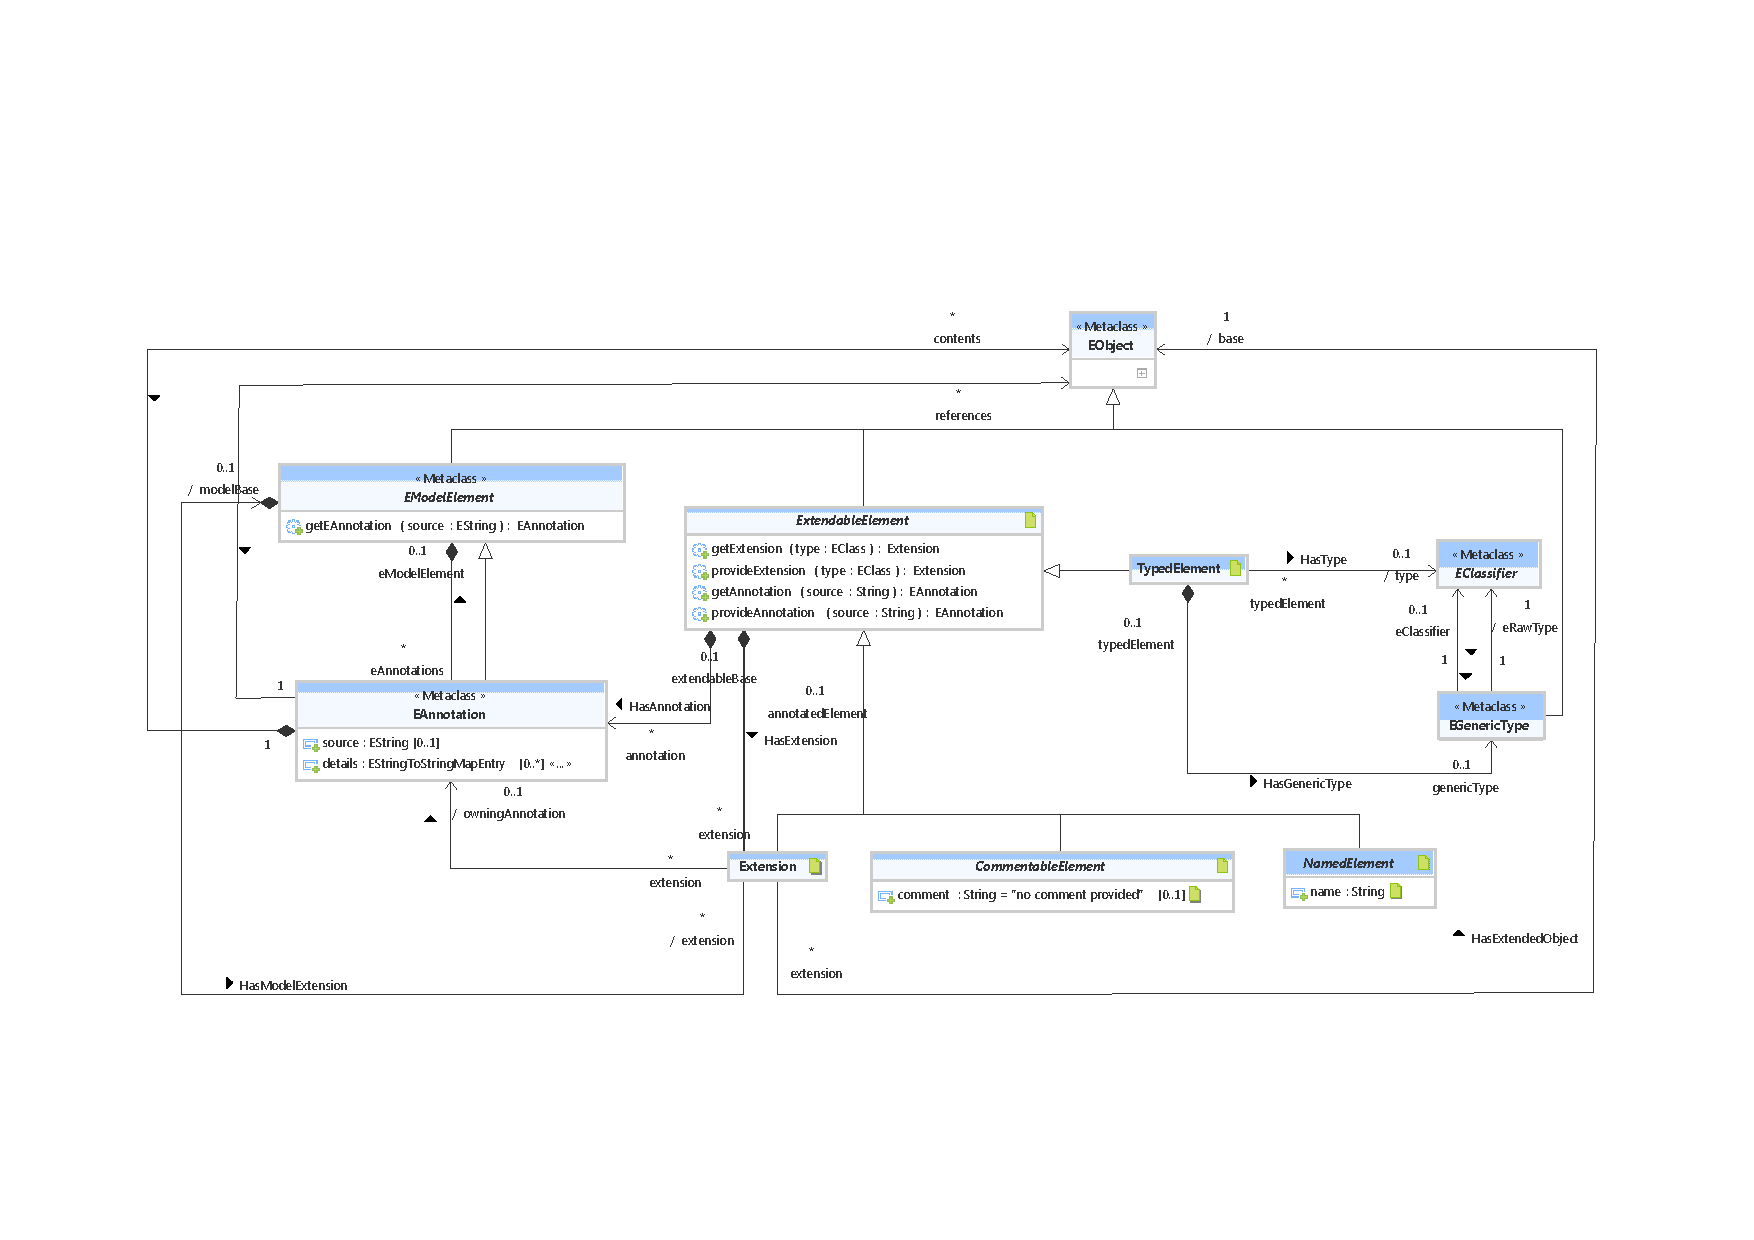
\includegraphics[width=\textheight,angle=90]{figures/A_technical-reference/packages/core/core}
  \caption{Class Structure of the \fe{core} Package}
  \label{fig:MM:modeling}
\end{figure}



\subsection{Detailed Contents Documentation}
\subsubsection{\Large{Class \bfseries \texttt{ArithmeticExpression}\normalfont}}
\label{cls:modeling::expressions::ArithmeticExpression} \index{8}
\paragraph{Overview}

	
			
Represents arithmetic expressions like a + 5 or a * 7.	
		
	


\begin{description}

	\item[\textbf{Class Properties}] Class \texttt{ArithmeticExpression} has the following properties:
	\begin{description}
\item[operator : ArithmeticOperator 	]
see Section~\ref{cls:modeling::expressions::ArithmeticOperator} on Page~\pageref{cls:modeling::expressions::ArithmeticOperator}\hspace{\fill}
\nopagebreak


	
			
Specifies the expression's arithmetic operator, e.g. +, -, *, /, or MODULO.	
		
	
	\end{description}
	
	

\end{description}

\paragraph{Parent Classes}
\begin{itemize}
\item BinaryExpression see Section~\ref{cls:modeling::expressions::BinaryExpression} on Page~\pageref{cls:modeling::expressions::BinaryExpression}\end{itemize}
\subsubsection{\Large{Enumeration \bfseries \texttt{ArithmeticOperator}\normalfont}}
\label{cls:modeling::expressions::ArithmeticOperator} \index{modeling::expressions!ArithmeticOperator}
\paragraph{Overview}
	
			
Defines the operators for arithmetic expressions.	
		
	


\begin{description}

	\item[\textbf{Enum Properties}] Enumeration \texttt{ArithmeticOperator} has the following literals:

	\begin{description}
		
		\item[PLUS = 0]
		\hspace{\fill}
		\nopagebreak

		\item[MINUS = 1]
		\hspace{\fill}
		\nopagebreak

		\item[TIMES = 2]
		\hspace{\fill}
		\nopagebreak

		\item[DIVIDE = 3]
		\hspace{\fill}
		\nopagebreak

		\item[MODULO = 4]
		\hspace{\fill}
		\nopagebreak

		\item[EXP = 5]
		\hspace{\fill}
		\nopagebreak
		
For formulas like a\^{}b.	
 
	\end{description}

\end{description}



\subsubsection{\Large{Class \bfseries \texttt{BinaryExpression}\normalfont}}
\label{cls:modeling::expressions::BinaryExpression} \index{6}
\paragraph{Overview}

	
			
Represents any binary expression like v < 5 or x + 7.	
		
	



\paragraph{Parent Classes}
\begin{itemize}
\item Expression see Section~\ref{cls:modeling::expressions::Expression} on Page~\pageref{cls:modeling::expressions::Expression}\end{itemize}
\subsubsection{\Large{Class \bfseries \texttt{BinaryLogicExpression}\normalfont}}
\label{cls:modeling::expressions::BinaryLogicExpression} \index{9}
\paragraph{Overview}

	
			
Represents binary, logic expressions like a AND b and a OR b.	
		
	


\begin{description}

	\item[\textbf{Class Properties}] Class \texttt{BinaryLogicExpression} has the following properties:
	\begin{description}
\item[operator : LogicOperator 	]
see Section~\ref{cls:modeling::expressions::LogicOperator} on Page~\pageref{cls:modeling::expressions::LogicOperator}\hspace{\fill}
\nopagebreak


	
			
Specifies the expression's logic operator, e.g. AND, OR, or XOR.	
		
	
	\end{description}
	
	

\end{description}

\paragraph{Parent Classes}
\begin{itemize}
\item BinaryExpression see Section~\ref{cls:modeling::expressions::BinaryExpression} on Page~\pageref{cls:modeling::expressions::BinaryExpression}\end{itemize}
\subsubsection{\Large{Enumeration \bfseries \texttt{ComparingOperator}\normalfont}}
\label{cls:modeling::expressions::ComparingOperator} \index{modeling::expressions!ComparingOperator}
\paragraph{Overview}
	
			
Defines the operators for comparing expressions.	
		
	


\begin{description}

	\item[\textbf{Enum Properties}] Enumeration \texttt{ComparingOperator} has the following literals:

	\begin{description}
		
		\item[LESS = 0]
		\hspace{\fill}
		\nopagebreak

		\item[LESS\_OR\_EQUAL = 1]
		\hspace{\fill}
		\nopagebreak

		\item[EQUAL = 2]
		\hspace{\fill}
		\nopagebreak

		\item[GREATER\_OR\_EQUAL = 3]
		\hspace{\fill}
		\nopagebreak

		\item[GREATER = 4]
		\hspace{\fill}
		\nopagebreak

		\item[UNEQUAL = 5]
		\hspace{\fill}
		\nopagebreak

		\item[REGULAR\_EXPRESSION = 6]
		\hspace{\fill}
		\nopagebreak
		
For comparison of a String with a regular expression.	
 
	\end{description}

\end{description}



\subsubsection{\Large{Class \bfseries \texttt{ComparisonExpression}\normalfont}}
\label{cls:modeling::expressions::ComparisonExpression} \index{7}
\paragraph{Overview}

	
			
Represents comparing expressions like a < 5 or a >= 7.	
		
	


\begin{description}

	\item[\textbf{Class Properties}] Class \texttt{ComparisonExpression} has the following properties:
	\begin{description}
\item[operator : ComparingOperator 	]
see Section~\ref{cls:modeling::expressions::ComparingOperator} on Page~\pageref{cls:modeling::expressions::ComparingOperator}\hspace{\fill}
\nopagebreak


	
			
Specifies the expression's comparing operator, e.g. <, >=, !=.	
		
	
	\end{description}
	
	

\end{description}

\paragraph{Parent Classes}
\begin{itemize}
\item BinaryExpression see Section~\ref{cls:modeling::expressions::BinaryExpression} on Page~\pageref{cls:modeling::expressions::BinaryExpression}\end{itemize}
\subsubsection{\Large{Class \bfseries \texttt{Expression}\normalfont}}
\label{cls:modeling::expressions::Expression} \index{10}
\paragraph{Overview}

	
			
Represents any expression in an embedded textual language, e.g. OCL or Java. An expression's type is dynamically derived by an external mechanism (see TypedElement).	
		
	



\paragraph{Parent Classes}
\begin{itemize}
\item TypedElement see Section~\ref{cls:modeling::TypedElement} on Page~\pageref{cls:modeling::TypedElement}, \item CommentableElement see Section~\ref{cls:modeling::CommentableElement} on Page~\pageref{cls:modeling::CommentableElement}\end{itemize}
\subsubsection{\Large{Class \bfseries \texttt{LiteralExpression}\normalfont}}
\label{cls:modeling::expressions::LiteralExpression} \index{4}
\paragraph{Overview}

	
			
Represents any literal, i.e. a value whose type is an EDataType. Literals are, for example, 5, 3.14, 'c', "text", true.	
		
	


\begin{description}

	\item[\textbf{Class Properties}] Class \texttt{LiteralExpression} has the following properties:
	\begin{description}
\item[value : EString 			\symbol{"5B}0..1\symbol{"5D}]
\hspace{\fill}
\nopagebreak


	
			
String representation of the value, e.g. "5", "3.14", "c", "text", or "true".	
		
	
	\end{description}
	
	\item[\textbf{Class References}] Class \texttt{LiteralExpression} has the following references:
	\begin{description}
\item[valueType : EDataType 	]
\hspace{\fill}
\nopagebreak


	
			
The literal's type, e.g. EInt, EString, etc.	
			
	
		
	
	\end{description}
	

\end{description}

\paragraph{Parent Classes}
\begin{itemize}
\item Expression see Section~\ref{cls:modeling::expressions::Expression} on Page~\pageref{cls:modeling::expressions::Expression}\end{itemize}
\subsubsection{\Large{Enumeration \bfseries \texttt{LogicOperator}\normalfont}}
\label{cls:modeling::expressions::LogicOperator} \index{modeling::expressions!LogicOperator}
\paragraph{Overview}
	
			
Defines the operators for binary logic expressions. The unary logic expression representing negated expressions is reflected by the NotExpression.	
		
	


\begin{description}

	\item[\textbf{Enum Properties}] Enumeration \texttt{LogicOperator} has the following literals:

	\begin{description}
		
		\item[AND = 0]
		\hspace{\fill}
		\nopagebreak

		\item[OR = 1]
		\hspace{\fill}
		\nopagebreak

		\item[XOR = 2]
		\hspace{\fill}
		\nopagebreak

		\item[IMPLY = 3]
		\hspace{\fill}
		\nopagebreak

		\item[EQUIVALENT = 4]
		\hspace{\fill}
		\nopagebreak
 
	\end{description}

\end{description}



\subsubsection{\Large{Class \bfseries \texttt{NotExpression}\normalfont}}
\label{cls:modeling::expressions::NotExpression} \index{5}
\paragraph{Overview}

	
			
Represents a negated expression, e.g. NOT (a < 5).	
		
	



\paragraph{Parent Classes}
\begin{itemize}
\item Expression see Section~\ref{cls:modeling::expressions::Expression} on Page~\pageref{cls:modeling::expressions::Expression}\end{itemize}
\subsubsection{\Large{Class \bfseries \texttt{TextualExpression}\normalfont}}
\label{cls:modeling::expressions::TextualExpression} \index{3}
\paragraph{Overview}

	
			
Represents any expression in a textual language embedded into Story Diagrams, e.g. OCL or Java .	
		
	


\begin{description}

	\item[\textbf{Class Properties}] Class \texttt{TextualExpression} has the following properties:
	\begin{description}
\item[expressionText : EString 	]
\hspace{\fill}
\nopagebreak


	
			
Holds the expression, e.g. in OCL or Java.	
		
	
\item[language : EString 	]
\hspace{\fill}
\nopagebreak


	
			
String representation of the used language which has to be unique. Examples are OCL and Java.	
		
	
\item[languageVersion : EString 			\symbol{"5B}0..1\symbol{"5D}]
\hspace{\fill}
\nopagebreak


	
			
String representation of the used language's version. The format is <Major>.<Minor>[.<Revision>[.<Build>]]
Examples: 1.4 or 3.0.1 or 1.0.2.20101208.	
		
	
	\end{description}
	
	

\end{description}

\paragraph{Parent Classes}
\begin{itemize}
\item Expression see Section~\ref{cls:modeling::expressions::Expression} on Page~\pageref{cls:modeling::expressions::Expression}\end{itemize}
\newpage
		


\section{Package \bfseries \texttt{modeling::patterns}\normalfont}
% Here comes the package documentation
\subsection{Package Overview}
	
			
This package contains all classes for modeling story patterns that may be 
embedded into StoryActivityNodes of an Activity.	
		
	
			
		
% Here a manual modifiable file is included: patterns/graphics.tex
%
% This file has been generated by Ecore to LaTeX written in oAW Xpand
% It is save to alter this file as it WILL NOT be overwritten.
% The file is included by the main latex file in the appropriate place, not further
% actions are required
%

\begin{figure}[htbp]
  \centering
  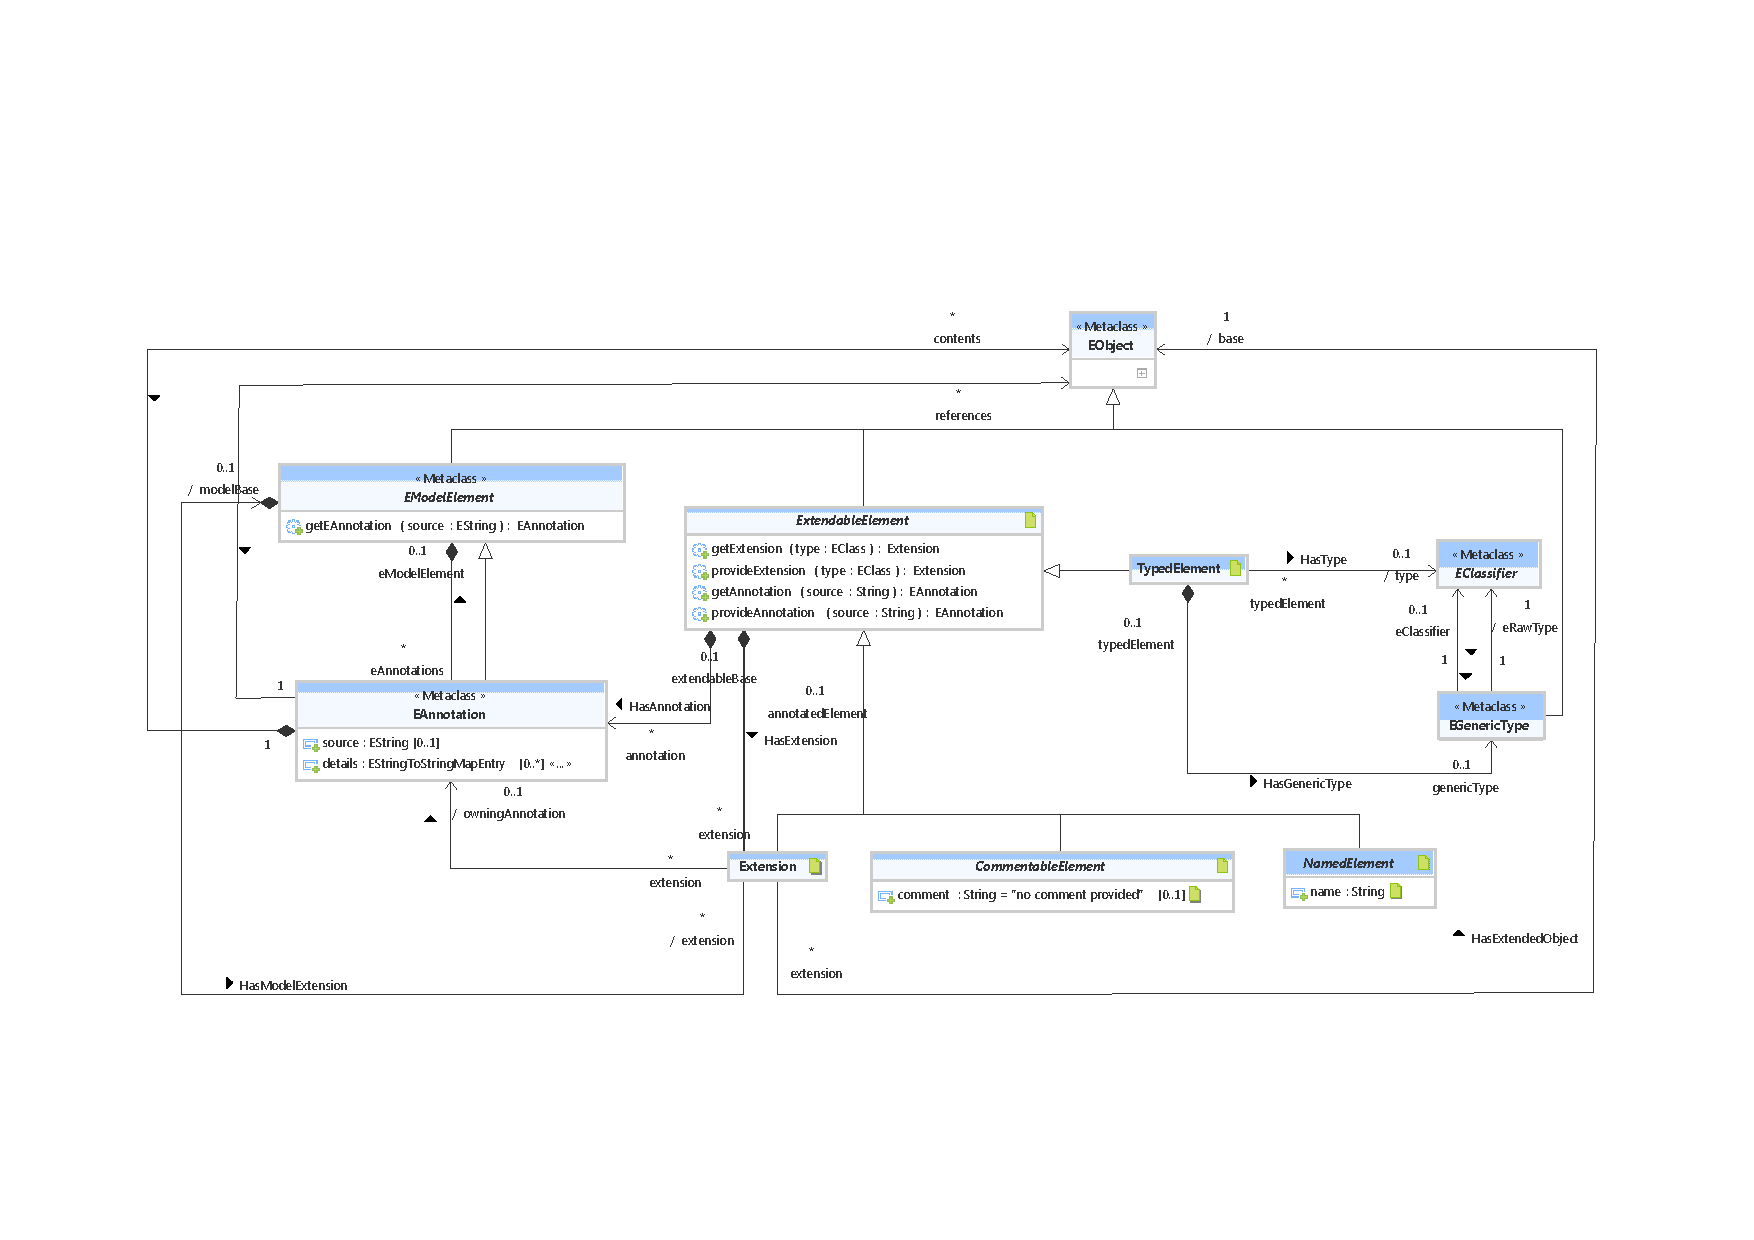
\includegraphics[width=\textheight,angle=90]{figures/A_technical-reference/packages/core/core}
  \caption{Class Structure of the \fe{core} Package}
  \label{fig:MM:modeling}
\end{figure}



\subsection{Detailed Contents Documentation}
\subsubsection{\Large{Class \bfseries \texttt{AbstractLinkVariable}\normalfont}}
\label{cls:modeling::patterns::AbstractLinkVariable} \index{4}
\paragraph{Overview}

	
			
Abstract super class for all kinds of link variables that represent links between two objects in a story pattern.	
		
	


\begin{description}

	\item[\textbf{Class Properties}] Class \texttt{AbstractLinkVariable} has the following properties:
	\begin{description}
\item[bindingOperator : BindingOperator 	]
see Section~\ref{cls:modeling::patterns::BindingOperator} on Page~\pageref{cls:modeling::patterns::BindingOperator}\hspace{\fill}
\nopagebreak


	
			
The binding operator defines whether this link will be matched, created or destroyed by the story pattern. The default value ist "check\_only", i.e., the link will be matched.	
		
	
\item[bindingSemantics : BindingSemantics 	]
see Section~\ref{cls:modeling::patterns::BindingSemantics} on Page~\pageref{cls:modeling::patterns::BindingSemantics}\hspace{\fill}
\nopagebreak


	
			
The binding semantics defines whether the link must be matched for a successful application of the containing story pattern, whether it must not be matched or whether it is optional, i.e., it will be bound if it can be bound but that does not affect the success of matching the story pattern. The default value is "mandatory" (i.e., it must be matched).	
		
	
\item[bindingState : BindingState 	]
see Section~\ref{cls:modeling::patterns::BindingState} on Page~\pageref{cls:modeling::patterns::BindingState}\hspace{\fill}
\nopagebreak


	
			
The binding state defines whether the link is already bound or whether a match has to be obtained for it.	
		
	
	\end{description}
	
	\item[\textbf{Class References}] Class \texttt{AbstractLinkVariable} has the following references:
	\begin{description}
\item[firstLinkConstraint : LinkConstraint 			\symbol{"5B}0..$*$\symbol{"5D}]
see Section~\ref{cls:modeling::patterns::LinkConstraint} on Page~\pageref{cls:modeling::patterns::LinkConstraint}\hspace{\fill}
\nopagebreak


		\todoib{Documentation missing?}
	
\item[pattern : StoryPattern 	]
see Section~\ref{cls:modeling::patterns::StoryPattern} on Page~\pageref{cls:modeling::patterns::StoryPattern}\hspace{\fill}
\nopagebreak


		\todoib{Documentation missing?}
	
\item[secondLinkConstraint : LinkConstraint 			\symbol{"5B}0..$*$\symbol{"5D}]
see Section~\ref{cls:modeling::patterns::LinkConstraint} on Page~\pageref{cls:modeling::patterns::LinkConstraint}\hspace{\fill}
\nopagebreak


		\todoib{Documentation missing?}
	
\item[source : ObjectVariable 	]
see Section~\ref{cls:modeling::patterns::ObjectVariable} on Page~\pageref{cls:modeling::patterns::ObjectVariable}\hspace{\fill}
\nopagebreak


		\todoib{Documentation missing?}
	
\item[target : AbstractVariable 	]
see Section~\ref{cls:modeling::patterns::AbstractVariable} on Page~\pageref{cls:modeling::patterns::AbstractVariable}\hspace{\fill}
\nopagebreak


		\todoib{Documentation missing?}
	
	\end{description}
	

\end{description}

\paragraph{Parent Classes}
\begin{itemize}
\item NamedElement see Section~\ref{cls:modeling::NamedElement} on Page~\pageref{cls:modeling::NamedElement}\end{itemize}
\subsubsection{\Large{Class \bfseries \texttt{AbstractVariable}\normalfont}}
\label{cls:modeling::patterns::AbstractVariable} \index{1}
\paragraph{Overview}

	
			
Abstract super class for object and primitive variables.	
		
	


\begin{description}

	\item[\textbf{Class Properties}] Class \texttt{AbstractVariable} has the following properties:
	\begin{description}
\item[bindingState : BindingState 	]
see Section~\ref{cls:modeling::patterns::BindingState} on Page~\pageref{cls:modeling::patterns::BindingState}\hspace{\fill}
\nopagebreak


	
			
The binding state defines whether the variable is already bound or whether a match has to be obtained for it. The default value is "unbound".	
		
	
	\end{description}
	
	\item[\textbf{Class References}] Class \texttt{AbstractVariable} has the following references:
	\begin{description}
\item[bindingExpression : Expression 			\symbol{"5B}0..1\symbol{"5D}]
see Section~\ref{cls:modeling::expressions::Expression} on Page~\pageref{cls:modeling::expressions::Expression}\hspace{\fill}
\nopagebreak


	
			
A binding expression can be used to bind a variable in a different way than just by pattern matching. This way, for example, the return value of a call can be bound to a variable.	
		
	
\item[constraint : Constraint 			\symbol{"5B}0..$*$\symbol{"5D}]
see Section~\ref{cls:modeling::patterns::Constraint} on Page~\pageref{cls:modeling::patterns::Constraint}\hspace{\fill}
\nopagebreak


	
			
All constraints which are defined for this variable. For a successful matching, all constraints for this variable must evaluate to true.	
		
	
\item[incomingLink : AbstractLinkVariable 			\symbol{"5B}0..$*$\symbol{"5D}]
see Section~\ref{cls:modeling::patterns::AbstractLinkVariable} on Page~\pageref{cls:modeling::patterns::AbstractLinkVariable}\hspace{\fill}
\nopagebreak


		\todoib{Documentation missing?}
	
\item[pattern : StoryPattern 	]
see Section~\ref{cls:modeling::patterns::StoryPattern} on Page~\pageref{cls:modeling::patterns::StoryPattern}\hspace{\fill}
\nopagebreak


		\todoib{Documentation missing?}
	
	\end{description}
	

\end{description}

\paragraph{Parent Classes}
\begin{itemize}
\item Variable see Section~\ref{cls:modeling::Variable} on Page~\pageref{cls:modeling::Variable}, \item NamedElement see Section~\ref{cls:modeling::NamedElement} on Page~\pageref{cls:modeling::NamedElement}\end{itemize}
\subsubsection{\Large{Class \bfseries \texttt{AttributeAssignment}\normalfont}}
\label{cls:modeling::patterns::AttributeAssignment} \index{9}
\paragraph{Overview}

	
			
An AttributeAssignment is used to set the value of a certain attribute of an object. It references the attribute that is to be set and the value. The value can be an expression to allow for calculations or calls that determine the final value. AttributeAssignments are carried out during the final phase of pattern application, i.e. after the matching and destruction are completed.	
		
	



\subsubsection{\Large{Enumeration \bfseries \texttt{BindingOperator}\normalfont}}
\label{cls:modeling::patterns::BindingOperator} \index{modeling::patterns!BindingOperator}
\paragraph{Overview}
	
			
The BindingOperator enum defines all possible operations for object and link variables. An object or link variable may be checked for existence be the story pattern (black object/link variable), it may be created (green object/link variable), or it may be destroyed (red object/link variable).	
		
	


\begin{description}

	\item[\textbf{Enum Properties}] Enumeration \texttt{BindingOperator} has the following literals:

	\begin{description}
		
		\item[CHECK\_ONLY = 0]
		\hspace{\fill}
		\nopagebreak
		
CHECK\_ONLY is the default value of this enum. It requires an object or link variable just to be matched by the story pattern.	

		\item[CREATE = 1]
		\hspace{\fill}
		\nopagebreak
		
An object or link variable marked as CREATE will be created by the story pattern.	

		\item[DESTROY = 2]
		\hspace{\fill}
		\nopagebreak
		
An object or link variable marked as DESTROY will be destroyed be the story pattern.	
 
	\end{description}

\end{description}



\subsubsection{\Large{Enumeration \bfseries \texttt{BindingSemantics}\normalfont}}
\label{cls:modeling::patterns::BindingSemantics} \index{modeling::patterns!BindingSemantics}
\paragraph{Overview}
	
			
The binding semantics defines which kind of match will be obtained for the object or link variable.	
		
	


\begin{description}

	\item[\textbf{Enum Properties}] Enumeration \texttt{BindingSemantics} has the following literals:

	\begin{description}
		
		\item[MANDATORY = 0]
		\hspace{\fill}
		\nopagebreak
		
For a mandatory object or link variable, a match has to be found for a pattern to be successfully applied.	

		\item[NEGATIVE = 1]
		\hspace{\fill}
		\nopagebreak
		
If an object or link variable is marked as NEGATIVE, no match may be found for that object or link variable. If a match can be found, the execution of the story pattern fails.	

		\item[OPTIONAL = 2]
		\hspace{\fill}
		\nopagebreak
		
For an OPTIONAL object or link variable, the matching tries to find a match. If no match can be found, this does not affect the success of the pattern application. If a match can be found, the respective object or link is bound to the variable.	
 
	\end{description}

\end{description}



\subsubsection{\Large{Enumeration \bfseries \texttt{BindingState}\normalfont}}
\label{cls:modeling::patterns::BindingState} \index{modeling::patterns!BindingState}
\paragraph{Overview}
	
			
The BindingState defines whether an object or link variable is already bound to a concrete value or not.	
		
	


\begin{description}

	\item[\textbf{Enum Properties}] Enumeration \texttt{BindingState} has the following literals:

	\begin{description}
		
		\item[UNBOUND = 0]
		\hspace{\fill}
		\nopagebreak
		
UNBOUND is the default value for this enum. If an object or link variable in a story pattern is unbound, a new match has to be obtained for that variable.	

		\item[BOUND = 1]
		\hspace{\fill}
		\nopagebreak
		
A bound variable has already been bound to a concrete value. The concrete value has to be passed either as a parameter or it has to be bound in a previous activity. If, during the execution of a story pattern, a bound variable has no value, the execution of the story pattern fails.	

		\item[MAYBE\_BOUND = 2]
		\hspace{\fill}
		\nopagebreak
		
A variable marked with maybe\_bound indicates that it is unknown (or unimportant) at design time whether the variable is bound or not. If, during the execution of the pattern, the variable is not bound, an object is matched and bound to the variable. If it is already bound, it is not altered. If the variable is still unbound after this process, the matching fails (except for OPTIONAL variables).	
 
	\end{description}

\end{description}



\subsubsection{\Large{Class \bfseries \texttt{Constraint}\normalfont}}
\label{cls:modeling::patterns::Constraint} \index{3}
\paragraph{Overview}

	
			
A constraint represents a condition which must be fulfilled for a successful pattern matching. It can either be contained in the story pattern or in a variable. In the former case, the constraint is evaluated after the matching of the object structure is complete. It still has to be true for the pattern application to be sucessful (and therefore for creations and destructions to be carried out). If the constraint is contained in a variable, it constrains the matching of that variable, i.e., it is evaluated during the matching of the containing variable and has to be true for a successful matching. If the variable is an ObjectSetVariable, the constraint has to be true for every object in the set.	
		
	



\subsubsection{\Large{Class \bfseries \texttt{ContainerVariable}\normalfont}}
\label{cls:modeling::patterns::ContainerVariable} \index{16}
\paragraph{Overview}

	
			
Represents a single container, e.g. a Set or List. ContainmentRelations can be used to add or remove objects to or from this container.
Every Constraint or AttributeAssignment can use the variable as a container (e.g., "set->size() > 5").	
		
	



\paragraph{Parent Classes}
\begin{itemize}
\item ObjectVariable see Section~\ref{cls:modeling::patterns::ObjectVariable} on Page~\pageref{cls:modeling::patterns::ObjectVariable}\end{itemize}
\subsubsection{\Large{Class \bfseries \texttt{ContainmentRelation}\normalfont}}
\label{cls:modeling::patterns::ContainmentRelation} \index{14}
\paragraph{Overview}

	
			
Specifies the containment of an object in a set (represented by a ContainerVariable). Will be displayed by a line having a circle with a plus inside at the end of the container (the source end of the link). A create modifier specifies that the object will be added to the container, delete that it will be removed, and none that it will be checked to be contained.	
		
	



\paragraph{Parent Classes}
\begin{itemize}
\item AbstractLinkVariable see Section~\ref{cls:modeling::patterns::AbstractLinkVariable} on Page~\pageref{cls:modeling::patterns::AbstractLinkVariable}\end{itemize}
\subsubsection{\Large{Class \bfseries \texttt{LinkConstraint}\normalfont}}
\label{cls:modeling::patterns::LinkConstraint} \index{7}
\paragraph{Overview}

	
			
Link constraints (formerly known as MultiLinks in old meta-model) constrain the ordering of links of the referencingObject is a collection. This way objects can be required to have a certain position in the collection (FIRST, LAST, INDEX) or a certain ordering relative to each other (DIRECT\_SUCCESSOR, INDIRECT\_SUCCESSOR). While the first kind of LinkConstraint can be imposed upon a single link, the second kind requires two links that are related to each other (e.g., have the same referencingObject).	
		
	


\begin{description}

	\item[\textbf{Class Properties}] Class \texttt{LinkConstraint} has the following properties:
	\begin{description}
\item[constraintType : LinkConstraintType 	]
see Section~\ref{cls:modeling::patterns::LinkConstraintType} on Page~\pageref{cls:modeling::patterns::LinkConstraintType}\hspace{\fill}
\nopagebreak


	
			
The constraint type of the LinkConstraint.	
		
	
\item[index : EInt 	]
\hspace{\fill}
\nopagebreak


	
			
The index of the linked object in the collection. The semantics of this attribute is only defined if the constraintType of the LinkConstraint is INDEX.	
		
	
\item[negative : EBoolean 	]
\hspace{\fill}
\nopagebreak


	
			
If the negative attribute is true, the link constraint may not be fulfilled for the complete pattern application to be successful.	
		
	
	\end{description}
	
	\item[\textbf{Class References}] Class \texttt{LinkConstraint} has the following references:
	\begin{description}
\item[firstLink : AbstractLinkVariable 	]
see Section~\ref{cls:modeling::patterns::AbstractLinkVariable} on Page~\pageref{cls:modeling::patterns::AbstractLinkVariable}\hspace{\fill}
\nopagebreak


		\todoib{Documentation missing?}
	
\item[referencingObject : ObjectVariable 	]
see Section~\ref{cls:modeling::patterns::ObjectVariable} on Page~\pageref{cls:modeling::patterns::ObjectVariable}\hspace{\fill}
\nopagebreak


		\todoib{Documentation missing?}
	
\item[secondLink : AbstractLinkVariable 			\symbol{"5B}0..1\symbol{"5D}]
see Section~\ref{cls:modeling::patterns::AbstractLinkVariable} on Page~\pageref{cls:modeling::patterns::AbstractLinkVariable}\hspace{\fill}
\nopagebreak


		\todoib{Documentation missing?}
	
	\end{description}
	

\end{description}

\paragraph{Parent Classes}
\begin{itemize}
\item ExtendableElement see Section~\ref{cls:modeling::ExtendableElement} on Page~\pageref{cls:modeling::ExtendableElement}\end{itemize}
\subsubsection{\Large{Enumeration \bfseries \texttt{LinkConstraintType}\normalfont}}
\label{cls:modeling::patterns::LinkConstraintType} \index{modeling::patterns!LinkConstraintType}
\paragraph{Overview}
	
			
The LinkConstraintType represents the different uses of LinkConstraints. Objects can be required to have a certain position in their containing collection (FIRST, LAST, INDEX) or a certain ordering relative to each other (DIRECT\_SUCCESSOR, INDIRECT\_SUCCESSOR).	
		
	


\begin{description}

	\item[\textbf{Enum Properties}] Enumeration \texttt{LinkConstraintType} has the following literals:

	\begin{description}
		
		\item[FIRST = 0]
		\hspace{\fill}
		\nopagebreak

		\item[LAST = 1]
		\hspace{\fill}
		\nopagebreak

		\item[DIRECT\_SUCCESSOR = 2]
		\hspace{\fill}
		\nopagebreak

		\item[INDIRECT\_SUCCESSOR = 3]
		\hspace{\fill}
		\nopagebreak

		\item[INDEX = 4]
		\hspace{\fill}
		\nopagebreak
 
	\end{description}

\end{description}



\subsubsection{\Large{Class \bfseries \texttt{LinkVariable}\normalfont}}
\label{cls:modeling::patterns::LinkVariable} \index{13}
\paragraph{Overview}

	
			
A link variable represents one link between two object variables. It is typed over one of the associations between the classes of those objects. Because EMF only directly supports references, the two link ends are typed over these references. In case of a uni-directional association, only the targetEnd is typed. In case of a bi-directional association, the reference that types the source end is automatically determined.	
		
	



\paragraph{Parent Classes}
\begin{itemize}
\item AbstractLinkVariable see Section~\ref{cls:modeling::patterns::AbstractLinkVariable} on Page~\pageref{cls:modeling::patterns::AbstractLinkVariable}\end{itemize}
\subsubsection{\Large{Class \bfseries \texttt{MatchingPattern}\normalfont}}
\label{cls:modeling::patterns::MatchingPattern} \index{15}
\paragraph{Overview}

	
			
A MatchingPattern is a special kind of story pattern that does not change the underlying graph. Thus, no contained object or link may carry an create or destroy BindingOperator.	
		
	



\paragraph{Parent Classes}
\begin{itemize}
\item StoryPattern see Section~\ref{cls:modeling::patterns::StoryPattern} on Page~\pageref{cls:modeling::patterns::StoryPattern}\end{itemize}
\subsubsection{\Large{Class \bfseries \texttt{ObjectSetVariable}\normalfont}}
\label{cls:modeling::patterns::ObjectSetVariable} \index{10}
\paragraph{Overview}

	
			
Represents a set of objects of the same type that are represented by a single node.
The context for contained Constraints and AttributeAssignments is every single object in the set. E.g., if the constraint is "name = 'abc'", only objects with that name are matched and added to the set. The use of the binding operator "CREATE" is not defined for ObjectSetVariables, i.e., the sets can only be matched and deleted.	
		
	



\paragraph{Parent Classes}
\begin{itemize}
\item ObjectVariable see Section~\ref{cls:modeling::patterns::ObjectVariable} on Page~\pageref{cls:modeling::patterns::ObjectVariable}\end{itemize}
\subsubsection{\Large{Class \bfseries \texttt{ObjectVariable}\normalfont}}
\label{cls:modeling::patterns::ObjectVariable} \index{0}
\paragraph{Overview}

	
			
An ObjectVariable holds a value of a complex type which is defined by an EClass. 	
		
	


\begin{description}

	\item[\textbf{Class Properties}] Class \texttt{ObjectVariable} has the following properties:
	\begin{description}
\item[bindingOperator : BindingOperator 	]
see Section~\ref{cls:modeling::patterns::BindingOperator} on Page~\pageref{cls:modeling::patterns::BindingOperator}\hspace{\fill}
\nopagebreak


	
			
The binding operator defines whether this object will be matched, created or destroyed by the story pattern.	
		
	
\item[bindingSemantics : BindingSemantics 	]
see Section~\ref{cls:modeling::patterns::BindingSemantics} on Page~\pageref{cls:modeling::patterns::BindingSemantics}\hspace{\fill}
\nopagebreak


	
			
The binding semantics defines whether the object must be matched for a successful application of the containing story pattern, whether it must not be matched or whether it is optional, i.e., it will be bound if it can be bound but that does not affect the success of matching the story pattern.	
		
	
	\end{description}
	
	\item[\textbf{Class References}] Class \texttt{ObjectVariable} has the following references:
	\begin{description}
\item[attributeAssignment : AttributeAssignment 			\symbol{"5B}0..$*$\symbol{"5D}]
see Section~\ref{cls:modeling::patterns::AttributeAssignment} on Page~\pageref{cls:modeling::patterns::AttributeAssignment}\hspace{\fill}
\nopagebreak


		\todoib{Documentation missing?}
	
\item[classifier : EClass 	]
\hspace{\fill}
\nopagebreak


	
			
The type of this ObjectVariable, given as an EClass.	
			
	
		
	
\item[linkOrderConstraint : LinkConstraint 			\symbol{"5B}0..$*$\symbol{"5D}]
see Section~\ref{cls:modeling::patterns::LinkConstraint} on Page~\pageref{cls:modeling::patterns::LinkConstraint}\hspace{\fill}
\nopagebreak


		\todoib{Documentation missing?}
	
\item[outgoingLink : AbstractLinkVariable 			\symbol{"5B}0..$*$\symbol{"5D}]
see Section~\ref{cls:modeling::patterns::AbstractLinkVariable} on Page~\pageref{cls:modeling::patterns::AbstractLinkVariable}\hspace{\fill}
\nopagebreak


		\todoib{Documentation missing?}
	
	\end{description}
	

\end{description}

\paragraph{Parent Classes}
\begin{itemize}
\item AbstractVariable see Section~\ref{cls:modeling::patterns::AbstractVariable} on Page~\pageref{cls:modeling::patterns::AbstractVariable}\end{itemize}
\subsubsection{\Large{Class \bfseries \texttt{Path}\normalfont}}
\label{cls:modeling::patterns::Path} \index{12}
\paragraph{Overview}

	
			
A path is a special link variable that specifies an indirect connection between two objects. That means, the connected objects have other links and objects "between them". Exactly which types of links may be traversed during the matching of a path can be constrained by a path expression.	
		
	



\paragraph{Parent Classes}
\begin{itemize}
\item AbstractLinkVariable see Section~\ref{cls:modeling::patterns::AbstractLinkVariable} on Page~\pageref{cls:modeling::patterns::AbstractLinkVariable}\end{itemize}
\subsubsection{\Large{Class \bfseries \texttt{PrimitiveVariable}\normalfont}}
\label{cls:modeling::patterns::PrimitiveVariable} \index{11}
\paragraph{Overview}

	
			
Represents a variable that holds a value of a primitive type, e.g. integer, boolean, String.	
		
	



\paragraph{Parent Classes}
\begin{itemize}
\item AbstractVariable see Section~\ref{cls:modeling::patterns::AbstractVariable} on Page~\pageref{cls:modeling::patterns::AbstractVariable}\end{itemize}
\subsubsection{\Large{Class \bfseries \texttt{StoryPattern}\normalfont}}
\label{cls:modeling::patterns::StoryPattern} \index{17}
\paragraph{Overview}

	
			
A Story Pattern is a graph rewrite rule that may be embedded into a StoryActivityNode
of an Activity.	
		
	


\begin{description}

	\item[\textbf{Class Properties}] Class \texttt{StoryPattern} has the following properties:
	\begin{description}
\item[bindingSemantics : BindingSemantics 	]
see Section~\ref{cls:modeling::patterns::BindingSemantics} on Page~\pageref{cls:modeling::patterns::BindingSemantics}\hspace{\fill}
\nopagebreak


		\todoib{Documentation missing?}
	
	\end{description}
	
	\item[\textbf{Class References}] Class \texttt{StoryPattern} has the following references:
	\begin{description}
\item[constraint : Constraint 			\symbol{"5B}0..$*$\symbol{"5D}]
see Section~\ref{cls:modeling::patterns::Constraint} on Page~\pageref{cls:modeling::patterns::Constraint}\hspace{\fill}
\nopagebreak


	
			
All constraints which are defined for this story pattern. For a successful matching, all constraints for this story pattern must evaluate to true.	
		
	
\item[containedPattern : StoryPattern 			\symbol{"5B}0..$*$\symbol{"5D}]
see Section~\ref{cls:modeling::patterns::StoryPattern} on Page~\pageref{cls:modeling::patterns::StoryPattern}\hspace{\fill}
\nopagebreak


		\todoib{Documentation missing?}
	
\item[linkVariable : AbstractLinkVariable 			\symbol{"5B}0..$*$\symbol{"5D}]
see Section~\ref{cls:modeling::patterns::AbstractLinkVariable} on Page~\pageref{cls:modeling::patterns::AbstractLinkVariable}\hspace{\fill}
\nopagebreak


		\todoib{Documentation missing?}
	
\item[parentPattern : StoryPattern 			\symbol{"5B}0..1\symbol{"5D}]
see Section~\ref{cls:modeling::patterns::StoryPattern} on Page~\pageref{cls:modeling::patterns::StoryPattern}\hspace{\fill}
\nopagebreak


		\todoib{Documentation missing?}
	
\item[templateSignature : TemplateSignature 			\symbol{"5B}0..1\symbol{"5D}]
see Section~\ref{cls:modeling::templates::TemplateSignature} on Page~\pageref{cls:modeling::templates::TemplateSignature}\hspace{\fill}
\nopagebreak


		\todoib{Documentation missing?}
	
\item[variable : AbstractVariable 			\symbol{"5B}0..$*$\symbol{"5D}]
see Section~\ref{cls:modeling::patterns::AbstractVariable} on Page~\pageref{cls:modeling::patterns::AbstractVariable}\hspace{\fill}
\nopagebreak


		\todoib{Documentation missing?}
	
	\end{description}
	

\end{description}

\paragraph{Parent Classes}
\begin{itemize}
\item CommentableElement see Section~\ref{cls:modeling::CommentableElement} on Page~\pageref{cls:modeling::CommentableElement}\end{itemize}
\newpage
		


\section{Package \bfseries \texttt{modeling::patterns::expressions}\normalfont}
% Here comes the package documentation
\subsection{Package Overview}
		\todoib{Documentation missing?}
	
			
		



\subsection{Detailed Contents Documentation}
\subsubsection{\Large{Class \bfseries \texttt{AttributeValueExpression}\normalfont}}
\label{cls:modeling::patterns::expressions::AttributeValueExpression} \index{0}
\paragraph{Overview}

	
			
Represents the value of an object's attribute, e.g. obj.attr for an object obj and an attribute attr.	
		
	



\paragraph{Parent Classes}
\begin{itemize}
\item Expression see Section~\ref{cls:modeling::expressions::Expression} on Page~\pageref{cls:modeling::expressions::Expression}\end{itemize}
\subsubsection{\Large{Class \bfseries \texttt{ObjectSetSizeExpression}\normalfont}}
\label{cls:modeling::patterns::expressions::ObjectSetSizeExpression} \index{2}
\paragraph{Overview}

	
			
Represents the number of elements in the set of objects that is represented by an object set variable. For example, if you have an object set variable mySet, then this expression would represent something like mySet.size(). The expression can be used to constrain the pattern application, e.g., to only a apply the pattern when at least two objects can be matched for the set.	
		
	



\paragraph{Parent Classes}
\begin{itemize}
\item Expression see Section~\ref{cls:modeling::expressions::Expression} on Page~\pageref{cls:modeling::expressions::Expression}\end{itemize}
\subsubsection{\Large{Class \bfseries \texttt{ObjectVariableExpression}\normalfont}}
\label{cls:modeling::patterns::expressions::ObjectVariableExpression} \index{1}
\paragraph{Overview}

	
			
Represents the reference to an object in an expression, i.e. the value of an object variable.	
		
	



\paragraph{Parent Classes}
\begin{itemize}
\item Expression see Section~\ref{cls:modeling::expressions::Expression} on Page~\pageref{cls:modeling::expressions::Expression}\end{itemize}
\subsubsection{\Large{Class \bfseries \texttt{PrimitiveVariableExpression}\normalfont}}
\label{cls:modeling::patterns::expressions::PrimitiveVariableExpression} \index{3}
\paragraph{Overview}

	
			
Represents the value of a primitive variable, e.g., 5 or "MyName".	
		
	



\paragraph{Parent Classes}
\begin{itemize}
\item Expression see Section~\ref{cls:modeling::expressions::Expression} on Page~\pageref{cls:modeling::expressions::Expression}\end{itemize}
\newpage
		


\section{Package \bfseries \texttt{modeling::templates}\normalfont}
% Here comes the package documentation
\subsection{Package Overview}
		\todoib{Documentation missing?}
	
			
		
% Here a manual modifiable file is included: templates/graphics.tex
%
% This file has been generated by Ecore to LaTeX written in oAW Xpand
% It is save to alter this file as it WILL NOT be overwritten.
% The file is included by the main latex file in the appropriate place, not further
% actions are required
%

\begin{figure}[htbp]
  \centering
  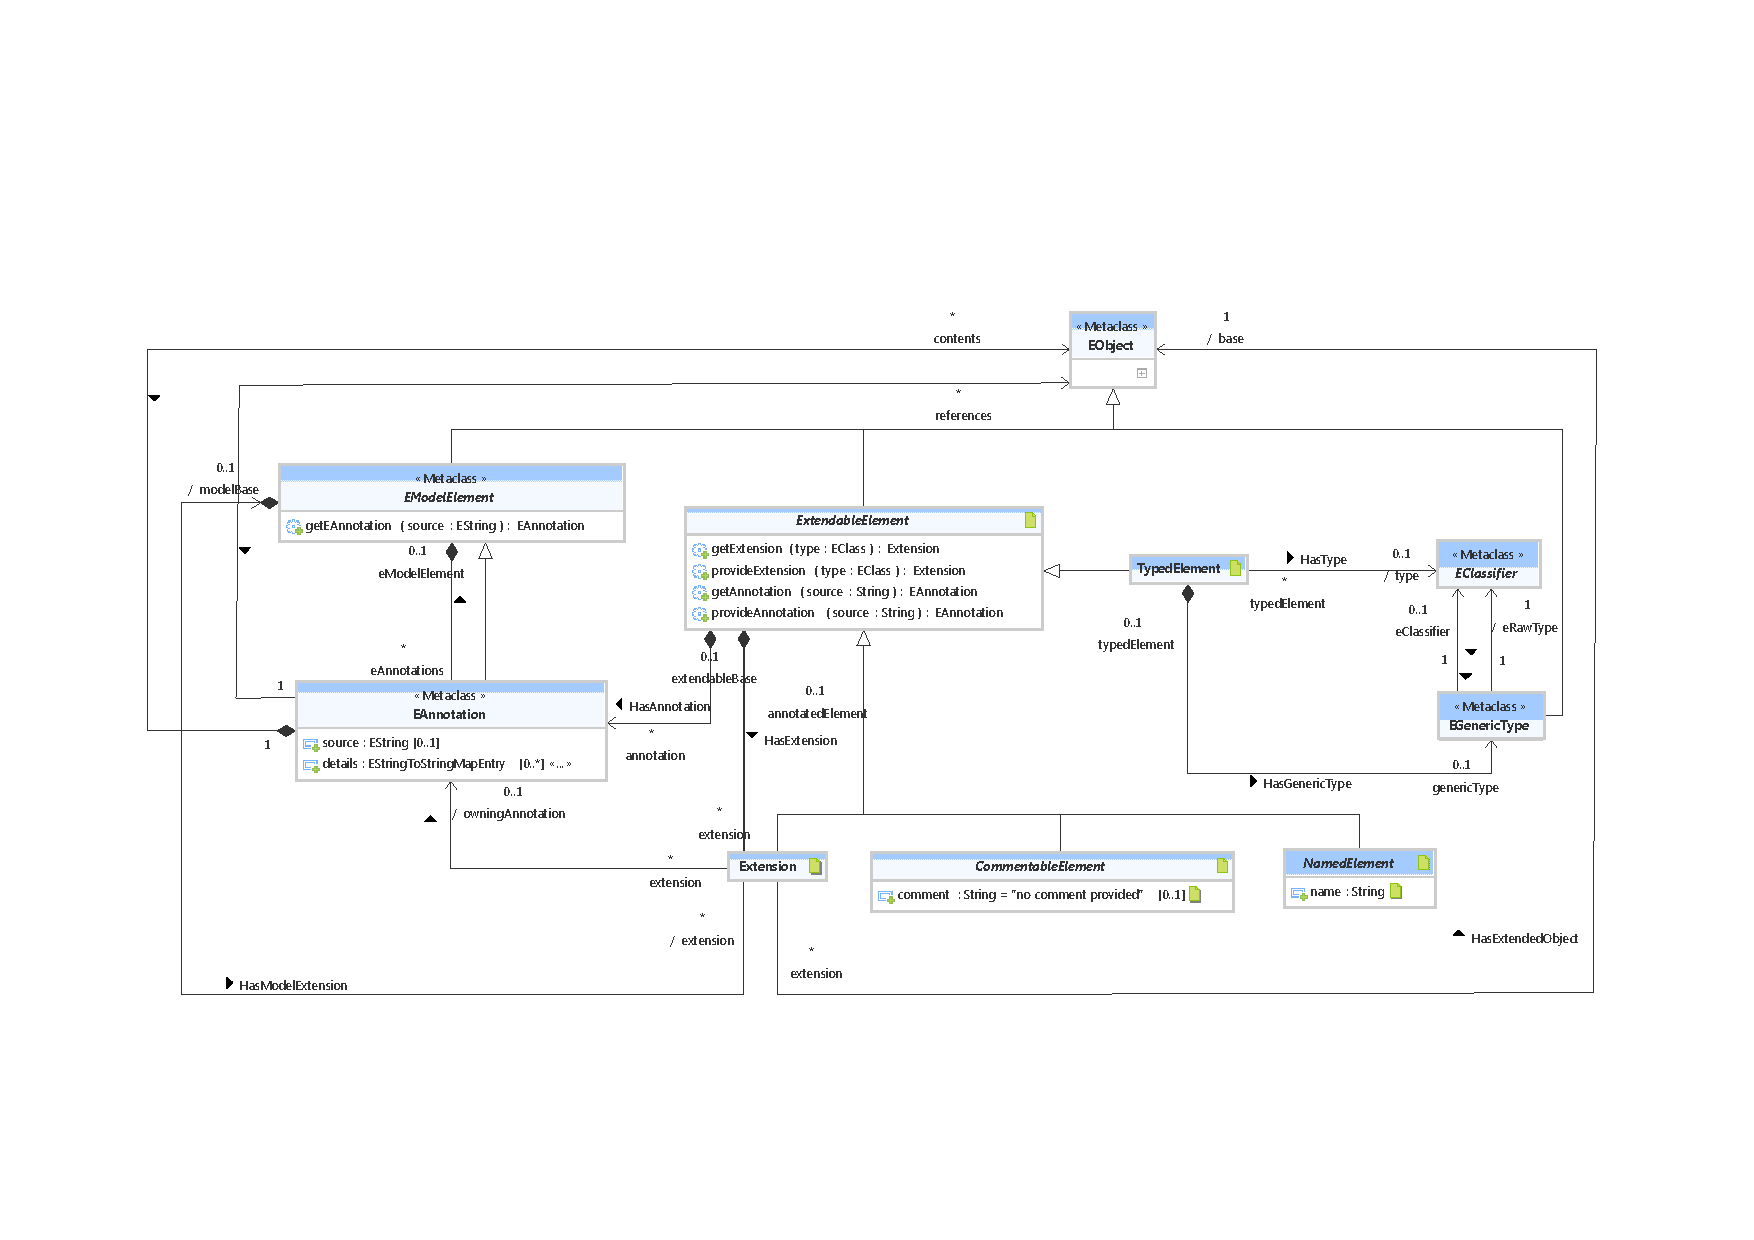
\includegraphics[width=\textheight,angle=90]{figures/A_technical-reference/packages/core/core}
  \caption{Class Structure of the \fe{core} Package}
  \label{fig:MM:modeling}
\end{figure}



\subsection{Detailed Contents Documentation}
\subsubsection{\Large{Class \bfseries \texttt{PropertyBinding}\normalfont}}
\label{cls:modeling::templates::PropertyBinding} \index{1}
\paragraph{Overview}

		\todoib{Documentation missing?}
	



\paragraph{Parent Classes}
\begin{itemize}
\item ExtendableElement see Section~\ref{cls:modeling::ExtendableElement} on Page~\pageref{cls:modeling::ExtendableElement}\end{itemize}
\subsubsection{\Large{Class \bfseries \texttt{TemplateBinding}\normalfont}}
\label{cls:modeling::templates::TemplateBinding} \index{0}
\paragraph{Overview}

		\todoib{Documentation missing?}
	



\paragraph{Parent Classes}
\begin{itemize}
\item ExtendableElement see Section~\ref{cls:modeling::ExtendableElement} on Page~\pageref{cls:modeling::ExtendableElement}\end{itemize}
\subsubsection{\Large{Class \bfseries \texttt{TemplateSignature}\normalfont}}
\label{cls:modeling::templates::TemplateSignature} \index{2}
\paragraph{Overview}

		\todoib{Documentation missing?}
	



\newpage
		




